\documentclass{beamer}
\usecolortheme{dolphin}
%\usetheme{Warsaw}

\usepackage{amsmath,amssymb,amsrefs}
\usepackage{amscd}
\usepackage{latexsym}
\usepackage{graphics}
\usepackage{subfigure}
\usepackage{placeins}
\usepackage{booktabs}
\usepackage{multirow}
\usepackage{bbm}
\usepackage{times}  % fonts are up to you
\usepackage[authoryear]{natbib}
\def\newblock{\hskip .11em plus .33em minus .07em} %this line is used to
% fix the bug of natbib that ``\newblock'' undefined.
\usepackage{array}

\usepackage{lipsum}
\usepackage{dsfont}

 \setbeamersize{text margin left=11pt,text margin right=8pt}
\newcommand\mydef{\mathrel{\overset{\makebox[0pt]{\mbox{\normalfont\tiny\sffamily def}}}{=}}}
\usepackage{soul}



\newif\ifpaper

% \papertrue % or
\paperfalse


\usepackage{graphicx}
\usepackage{nicefrac}
\usepackage{lscape}
\usepackage{times}
% \usepackage[dvips,colorlinks=true,linkcolor=red,filecolor=green,citecolor=red]{hyperref}
%\usepackage[]{amsmath,amssymb,epsfig}
% \usepackage{subfigure}
\usepackage{mathtools}%
\usepackage{algorithm}
\usepackage{algorithmic}
\usepackage{wrapfig}





\newcommand{\mb}[1]{\mbox{\boldmath$#1$}}

\setbeamertemplate{headline}{\scriptsize{\vspace*{0.1cm}\hspace*{0.1cm}\insertframenumber}}

\title{Centrality Measure Based on Clusterings in the Effective Resistance Embedding Space}
\author{Kevin Bui, Joe Feng, Alto Senda, Justin Wang\\
\vspace{5mm}
MATH 191 Graphs and Networks, UCLA}
% \institute[]{ Applied Mathematics, UCLA
% Applied and Computational Mathematics, \\
% Princeton University
% }
%\address{PACM Graduate Student Seminar}
% \date{ Harvard University \\ February 24, 2014}

\date{ \today}

% note: do NOT include a \maketitle line; also note that this title
% material goes BEFORE the \begin{document}

%%%%% have this if you'd like a recurring outline
\AtBeginSection[]  % "Beamer, do the following at the start of every section"
{
\begin{frame}<beamer>
  \frametitle{Outline} % make a frame titled "Outline"
  \tableofcontents[currentsection]  % show TOC and highlight current section
\end{frame}
}


\begin{document}

\newtheorem{theo}{Theorem}
\newtheorem{lem}{Lemma}
\newtheorem{defin}{Definition}
\newtheorem{prop}{Proposition}
\newtheorem{ex}{Example}
\newtheorem{alg}{Algorithm}
\newtheorem{cor}{Corollary}
\newtheorem{case}{Case}


% this prints title, author etc. info from above
\begin{frame}
  \titlepage
\end{frame}



\section{Introduction}

\begin{frame}
     \frametitle{Introduction}
In our project:
\begin{itemize}
\item Review betweenness and closeness centrality measures.
\item Introduce their variants and concept of electrical resistance embedding when visualizing a graph as an electrical network.
\item Apply $k$-means algorithm on the effective resistance embedding to create a new centrality measure called $k$-means centrality.
\item Compare the proposed $k$-means centrality to the existing centrality measures to see how discriminative it is for the nodes of the graph 
\end{itemize}

\end{frame}


\section{Centrality Measures}    \label{sec:ourWork}

\begin{frame}
     \frametitle{Review of Centrality Measure}
Recall that:
\begin{itemize}
\item Centrality measures attempt to quantify the importance of nodes, edges, or other network structures.
\item A good choice of centrality measure depends on context; what does it mean to be "most central"?
\item A slight change to the definition of a centrality measure can have large changes.
\end{itemize}
\end{frame}

\begin{frame}
     \frametitle{Betweenness Centrality}
     Betweenness centrality measures the extent on which a node lies on the shortest path of a graph.\\
     \vspace{5mm}
     It is defined as follows:
     \begin{align*}
      c_{B}(v)=\frac{1}{n_{B}} \sum_{s,t \in V} \frac{\sigma_{st}(v)}{\sigma_{s,t}}
     \end{align*}
     where 
     \begin{itemize}
     \item $n_B = n(n-1)$ such that $n$ is the number of nodes of a graph.
     \item $\sigma_{st}(v)$ denotes the number of shortest paths from $s$ to $t$ containing $v$.
     \item $\sigma_{s,t}$ denotes the number of shortest paths from $s$ to $t$.
     \end{itemize}
\end{frame}


\begin{frame}
     \frametitle{Closeness Centrality}
     Closeness centrality is based on the .\\
     \vspace{5mm}
     Closeness centrality is defined as:
     \begin{align*}
     c_{C}(v)=\frac{n_{C}}{\sum\limits_{t\neq v} d_{G}(v,t)}
     \end{align*}
     where
     \begin{itemize}
     \item $n_C = n-1$.
     \item $d_{G}(v,t)$ denotes the length of a shortest path between $v$ and $t$.
     \end{itemize}
\end{frame}


%\begin{frame}
%     \frametitle{Weakness of Closeness Centrality}
%     \begin{itemize}
%     \item It is difficult to distinguish between central %and less central nodes using this measure
%     \item For large network, the ratio of largest and %smallest closeness centrality is small, which is not easy %to see the difference for other nodes
%     \item nodes in small component get higher %closeness centrality than the nodes in larger components
%     \end{itemize}
%\end{frame}


\begin{frame}
     \frametitle{Graph as an Electrical Network}
     We may view the graph as an electrical network by corresponding  the weight of each edge as the conductance. Since we are working with unweighted graphs, the conductance of each edge is $1$.\\
    \vspace{5mm}
    The supply vector $b: V \rightarrow \mathbb{R}$ defines where current externally enters and leaves the network. For our case, if node $s$ is the source and node $t$ is the sink of the current, then we have
          \begin{align*}
     b_{st}(v) =
\begin{cases}
1, & \text{if }v=s 
\\
-1, & \text{if }v=t
\\
0 & \text{otherwise}
\end{cases}
     \end{align*}

Each edge is given an arbitrary orientation to account for direction of flow.
The vector $x: \vec{E} \rightarrow \mathbb{R}$ is defined to be the current of the network.
\end{frame}


\begin{frame}
     \frametitle{Graph as an Electrical Network}
         \begin{figure}[h]
\begin{center}
\includegraphics[width=0.76\columnwidth]{current_flow}
\end{center}
\caption{A simple electrical circuit}
\label{fig:A simple electrical circuit}
\end{figure}
\end{frame}



\begin{frame}
     \frametitle{Graph as an Electrical Network}
          Currents are related to voltages or potential differences $\hat{p}:\vec{E} \rightarrow \mathbb{R}$ by $\hat{p}(\vec{e}) = x(\vec{e})$ for all $e \in E$, so the absolute potential of $p: V \rightarrow \mathbb{R}$ is assigned when $\hat{p}(v,w) = p(v) - p(w)$ for all $(v,w) \in \vec{E}$.\\
     \vspace{5mm}The absolute potentials can be computed directly by the system 
     \begin{align*}
     Lp = b 
     \end{align*}
     where $L = D-A$ as the Laplacian matrix. \\
     \vspace{5mm}
     Since $L$ is singular, we fix $p(v_1) = 0$ so that we have the following: 
     \begin{align*}
     p = \left( \begin{array}{cc}
0 & \mathbf{0}^T \\
\mathbf{0} & \widetilde{L}^{-1} \\
\end{array} \right) b
     \end{align*} where $\widetilde{L} \in \mathbb{R}^{n-1 \times n-1}$ is the matrix obtained from $L$ by omitting the row and column of $v_1$.
\end{frame}
\begin{frame}{Current-Flow Betweenness Centrality}
In an electrical network, the analog of the fraction of shortest $st$-paths passing through a node is the fraction of a unit $st$-current flowing through it. \\
\vspace{5mm}
Given a supply $b$ under a $st$-current, the throughput of a node $v \in V$ is defined as
\begin{align*}
\tau_{st}(v) = \frac{1}{2}\left( -\left|b(v) \right| + \sum_{e: v \in e} \left|x(\vec{e})\right|\right).
\end{align*}
The current-flow betweenness centrality is defined as
\begin{align*}
c_{CB}(v) = \frac{1}{n_B} \sum_{s,t \in V} \tau_{st}(v)
\end{align*}
where $n_B = (n-1)(n-2)$.
\end{frame}
\begin{frame}
\frametitle{Current-Flow Closeness Centrality}
To introduce the variant of closeness centrality on an electrical network, the current-flow closeness centrality is defined as follows:
\begin{align*}
c_{CC}(s) = \frac{n_C}{\displaystyle \sum_{t \neq s} p_{st}(s) - p_{st}(t)}
\end{align*}
where $n_C = n-1$.\\
\vspace{5mm}
Here $p_{st}(s) - p_{st}(t)$ is the effective resistance, which is an alternative measure of distance between $s$ and $t$. We need an efficient way of computing it between each pair of nodes.
\end{frame}

\begin{frame}{Effective Resistance}
Spielman-Srivastava proposed the following method to approximate effective resistances:
\begin{enumerate}
\item Solve the systems $LX = B^TQ$
\item Effective resistance between nodes $s$ and $t$ is equal to $\|X_s - X_j\|_2$ where $X_i$ is the $i$th row of $X$.
\end{enumerate}
where
\begin{itemize}
\item $L$ is the Laplacian
\item $B$ is the incident matrix
\item $Q$ is the random Johnson-Lindenstrauss projection of size $m \times O(\textrm{log }n)$.
\end{itemize}
$X$ is called the effective resistance embedding since each row corresponds to a node embedded in $n \times O(\textrm{log }n)$-dimensional Euclidean space. We can apply $k$-means to it.
\end{frame}

\begin{frame}{$k$-means Clustering}
$k$-means clustering is the most basic but most widely used clustering technique. It partitions a dataset into $k$ clusters \{$S_1, S_2, ..., S_k$\}. \\
\bigskip\noindent
The algorithm is as follows:
\begin{enumerate}
\item Randomly pick $k$ data points and initialize them as centroids. 
\item Calculate the distance between each data point to each centroid.
\item Assign each data point to the closet centroid. 
\item Compute new centroids by calculating the mean of the data points in each cluster.
\item Repeat Steps 2-4 until convergence.
\end{enumerate}
\end{frame}

\begin{frame}{$k$-Means Centrality}
We propose a new centrality measure based on applying $k$-means to effective resistance embedding. It is defined as the following:
\begin{align*}
c_{K}(s) = \sum_{k = 2}^L \sum_{t\in V} \mathbbm{1} _{\{\textrm{edge $st$ is a cut edge in a $k$-clustering on $\{S_1^{(k)}, S_2^{(k)}, ..., S_k^{(k)}\}$}\}}.
\end{align*}
The cut edge is defined as an edge whose endpoints lie in two different partition sets and $\mathbbm{1}$ is the indicator function.
\end{frame}

\section{Numerical Experiments on Synthetic Data}  \label{sec:NumExpSyn}

\begin{frame}
\frametitle{Numerical Experiments on Synthetic Data}
\begin{itemize}
\item We implement the centrality measures on two toy data sets. 
\begin{columns}[T]
\begin{column}{.5\textwidth}
\begin{figure}[h]
\begin{center}
\includegraphics[width=0.76\columnwidth]{toy1.png}
\end{center}
\caption{Toy Network}
\label{fig:Toy}
\end{figure}
\end{column}
\begin{column}{.5\textwidth}
\begin{figure}[h]
\begin{center}
\includegraphics[width=0.76\columnwidth]{tripartite.png}
\end{center}
\caption{"Tripartite" Graph}
\label{fig:Toy2}
\end{figure}
\end{column}
\end{columns}
\item For the following graphs, note that nodes with higher centrality measures are larger and are closer to violet on the spectrum and nodes with lower centrality measures are smaller and are closer to red on the spectrum.
\end{itemize}
\end{frame}


%\begin{frame}
%\frametitle{Numerical experiments on synthetic data}
%\begin{itemize}
%\item Closeness Centrality (Toy network)
%\begin{figure}[h]
%\begin{center}
%\includegraphics[width=0.76\columnwidth]{toy_closeness}
%\end{center}
%\caption{Closeness Centrality of network Toy}
%\label{fig:Closeness Centrality - Toy}
%\end{figure}
%\end{itemize}
%\end{frame}

%\begin{frame}
%\frametitle{Numerical experiments on synthetic data}
%\begin{itemize}
%\item Betweenness Centrality (Toy network)
%\begin{figure}[h]
%\begin{center}
%\includegraphics[width=0.76\columnwidth]{toy_betweenness}
%\end{center}
%\caption{Betweenness Centrality of network Toy}
%\label{fig:Betweenness Centrality - Toy}
%\end{figure}
%\end{itemize}
%\end{frame}


%\begin{frame}
%\frametitle{Numerical experiments on synthetic data}
%\begin{itemize}
%\item Current Flow Closeness Centrality (Toy network)
%\begin{figure}[h]
%\begin{center}
%\includegraphics[width=0.76\columnwidth]{toy_current_flow_closeness}
%\end{center}
%\caption{Current Flow Closeness Centrality of network Toy}
%\label{fig:Current Flow Closeness Centrality - Toy}
%\end{figure}
%\end{itemize}
%\end{frame}

%\begin{frame}
%\frametitle{Numerical experiments on synthetic data}
%\begin{itemize}
%\item Current Flow Betweenness Centrality (Toy network)
%\begin{figure}[h]
%\begin{center}
%\includegraphics[width=0.76\columnwidth]{toy_current_flow_betweenness}
%\end{center}
%\caption{Current Flow Betweenness Centrality of network Toy}
%\label{fig:Current Flow Betweenness Centrality - Toy}
%\end{figure}
%\end{itemize}
%\end{frame}

\begin{frame}
\frametitle{Numerical Experiments on Synthetic Data}
\begin{columns}[T]
\begin{column}{.5\textwidth}
\begin{figure}[h]
\begin{center}
\includegraphics[width=0.76\columnwidth]{toy_closeness}
\end{center}
\caption{Closeness Centrality of Toy Network}
\label{fig:Closeness Centrality - Toy}
\end{figure}
\end{column}
\begin{column}{.5\textwidth}
\begin{figure}[h]
\begin{center}
\includegraphics[width=0.76\columnwidth]{toy_current_flow_closeness}
\end{center}
\caption{Current-Flow Closeness Centrality of Toy Network}
\label{fig:Current Flow Closeness Centrality - Toy}
\end{figure}
\end{column}
\end{columns}
\end{frame}

\begin{frame}
\frametitle{Numerical Experiments on Synthetic Data}
\begin{columns}[T]
\begin{column}{.5\textwidth}
\begin{figure}[h]
\begin{center}
\includegraphics[width=0.76\columnwidth]{toy_betweenness}
\end{center}
\caption{Betweenness Centrality of Toy Network}
\label{fig:Betweenness Centrality - Toy}
\end{figure}
\end{column}
\begin{column}{.5\textwidth}
\begin{figure}[h]
\begin{center}
\includegraphics[width=0.76\columnwidth]{toy_current_flow_betweenness}
\end{center}
\caption{Current-Flow Betweenness Centrality of Toy Network}
\label{fig:Current Flow Betweenness Centrality - Toy}
\end{figure}
\end{column}
\end{columns}
\end{frame}

\begin{frame}
\frametitle{Numerical Experiments on Synthetic Data}
\begin{figure}[h]
\begin{center}
\includegraphics[width=0.76\columnwidth]{toy_k_centrality}
\end{center}
\caption{$k$-Means Centrality of Toy Network}
\label{fig:K-Centrality - Toy}
\end{figure}
\end{frame}


\begin{frame}
\frametitle{Numerical Experiments on Synthetic Data}
\begin{figure}[h]
\begin{center}
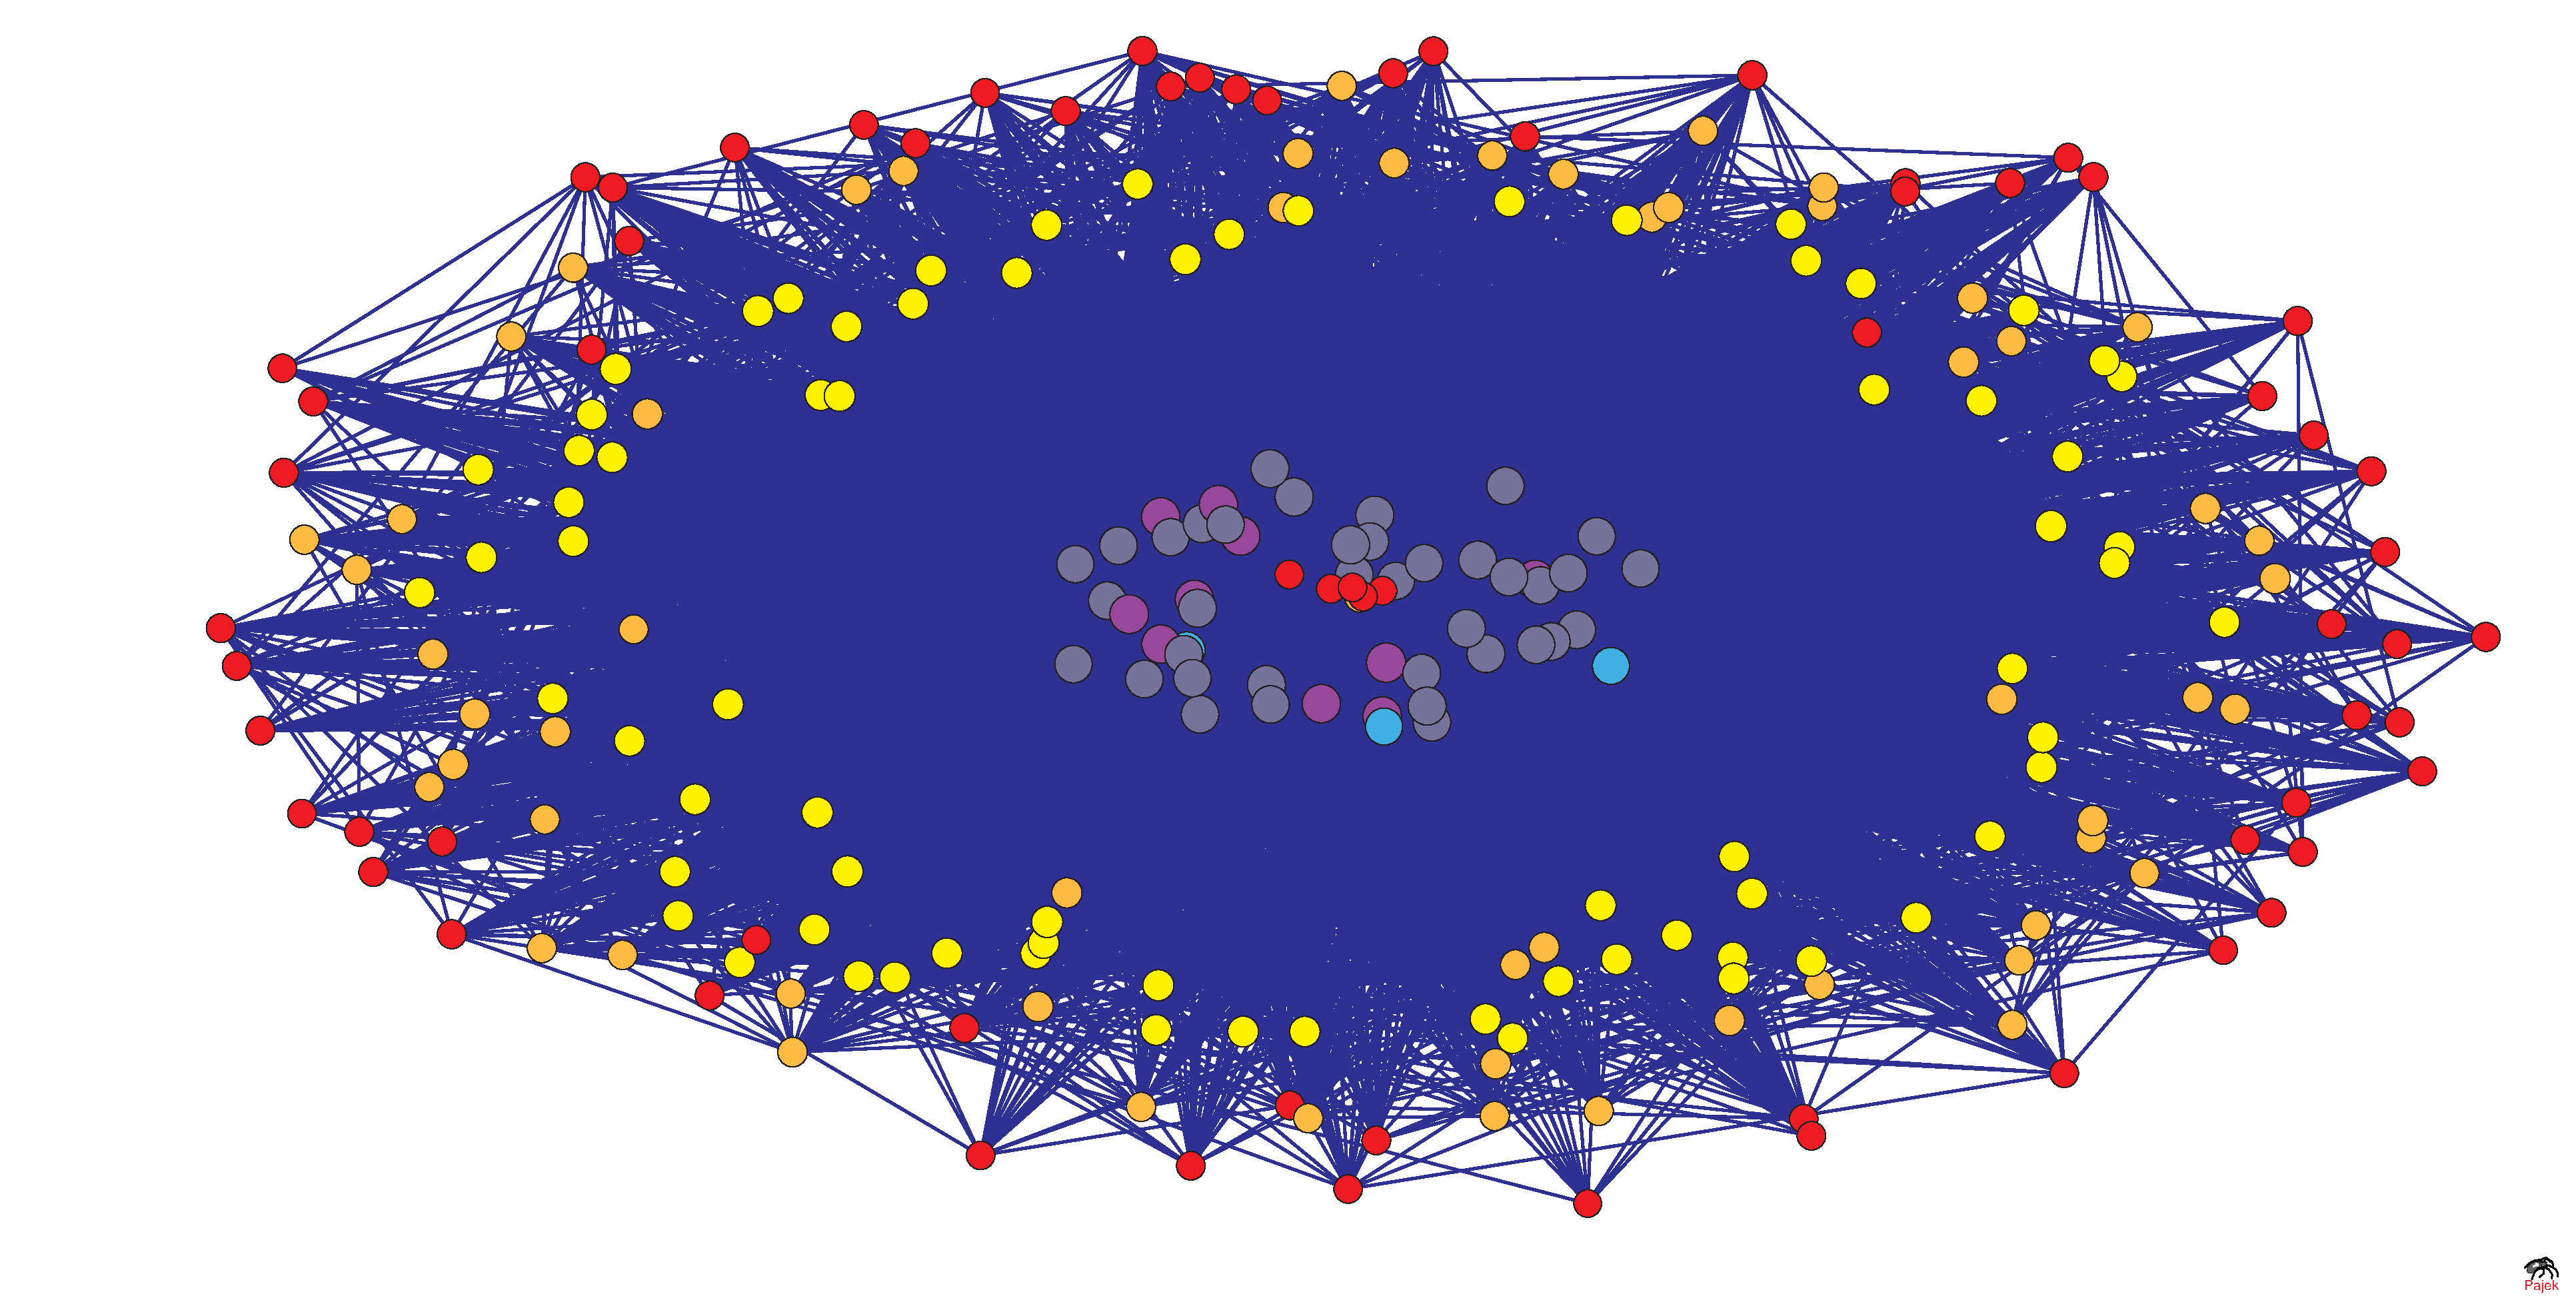
\includegraphics[width=0.76\columnwidth]{toy2_closeness2}
\end{center}
\caption{Closeness Centrality of "Tripartite" Graph}
\label{fig:Closeness Centrality - Toy2}
\end{figure}
\end{frame}

\begin{frame}
\frametitle{Numerical Experiments on Synthetic Data}
\begin{figure}[h]
\begin{center}
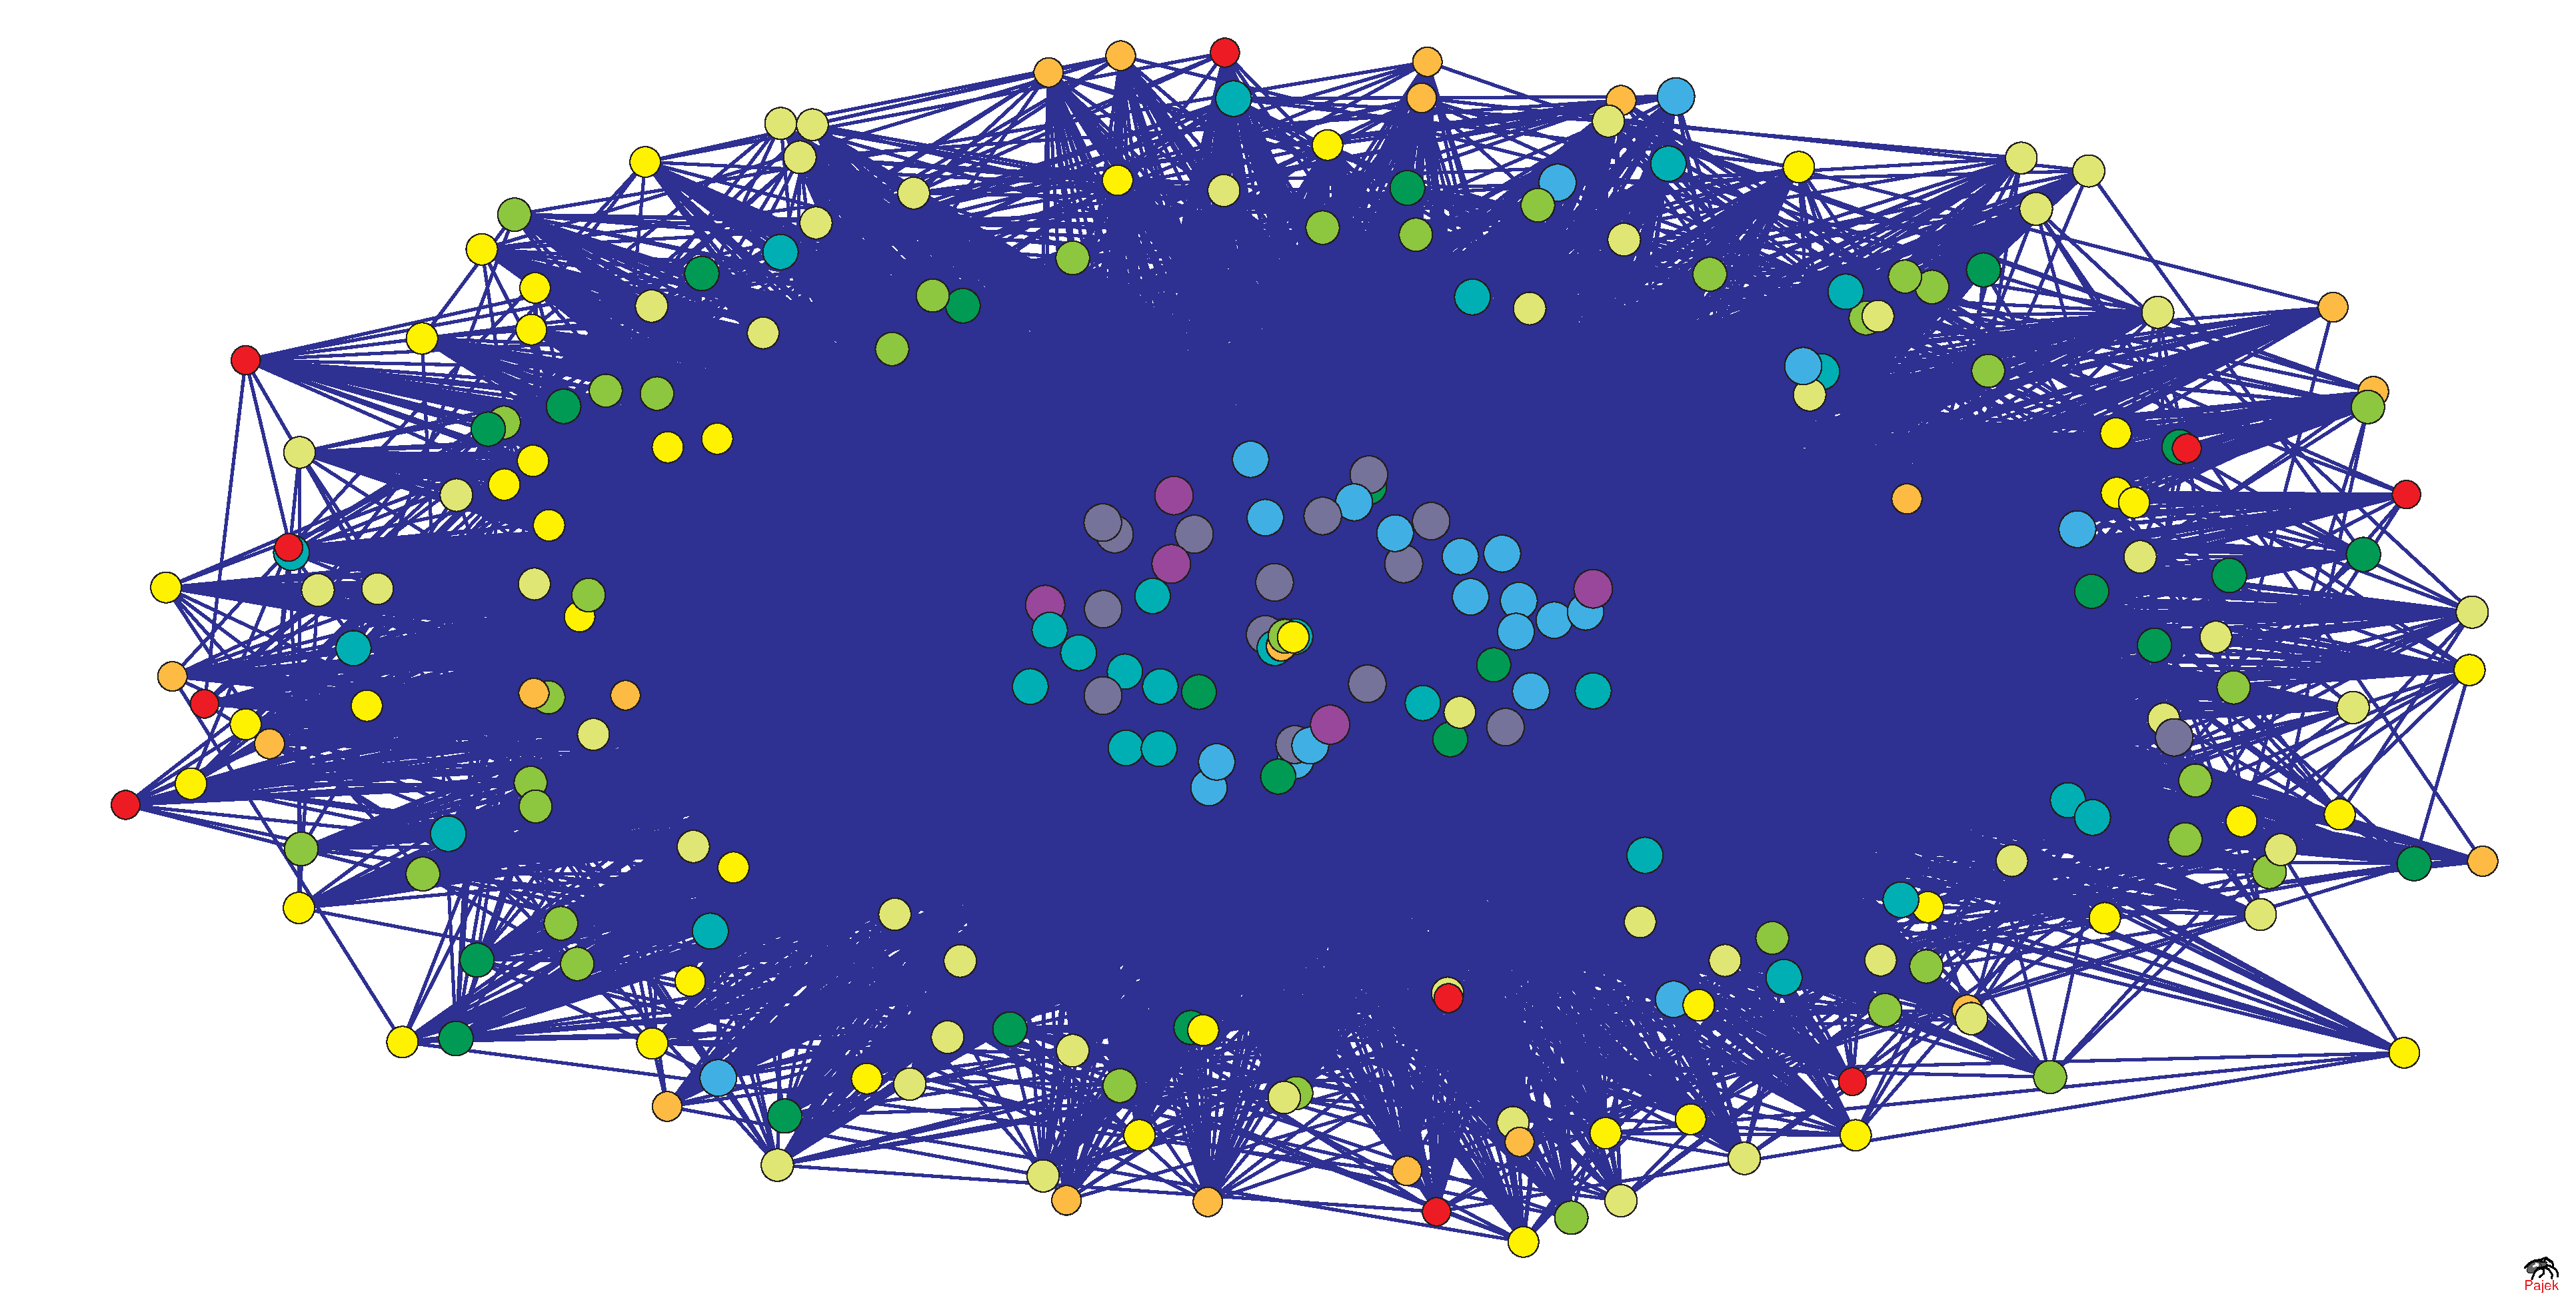
\includegraphics[width=0.76\columnwidth]{toy2_current_flow_closeness}
\end{center}
\caption{Current-Flow Closeness Centrality of "Tripartite" Graph}
\label{fig:Current Flow Closeness Centrality - Toy2}
\end{figure}
\end{frame}

\begin{frame}
\frametitle{Numerical Experiments on Synthetic Data}
\begin{figure}[h]
\begin{center}
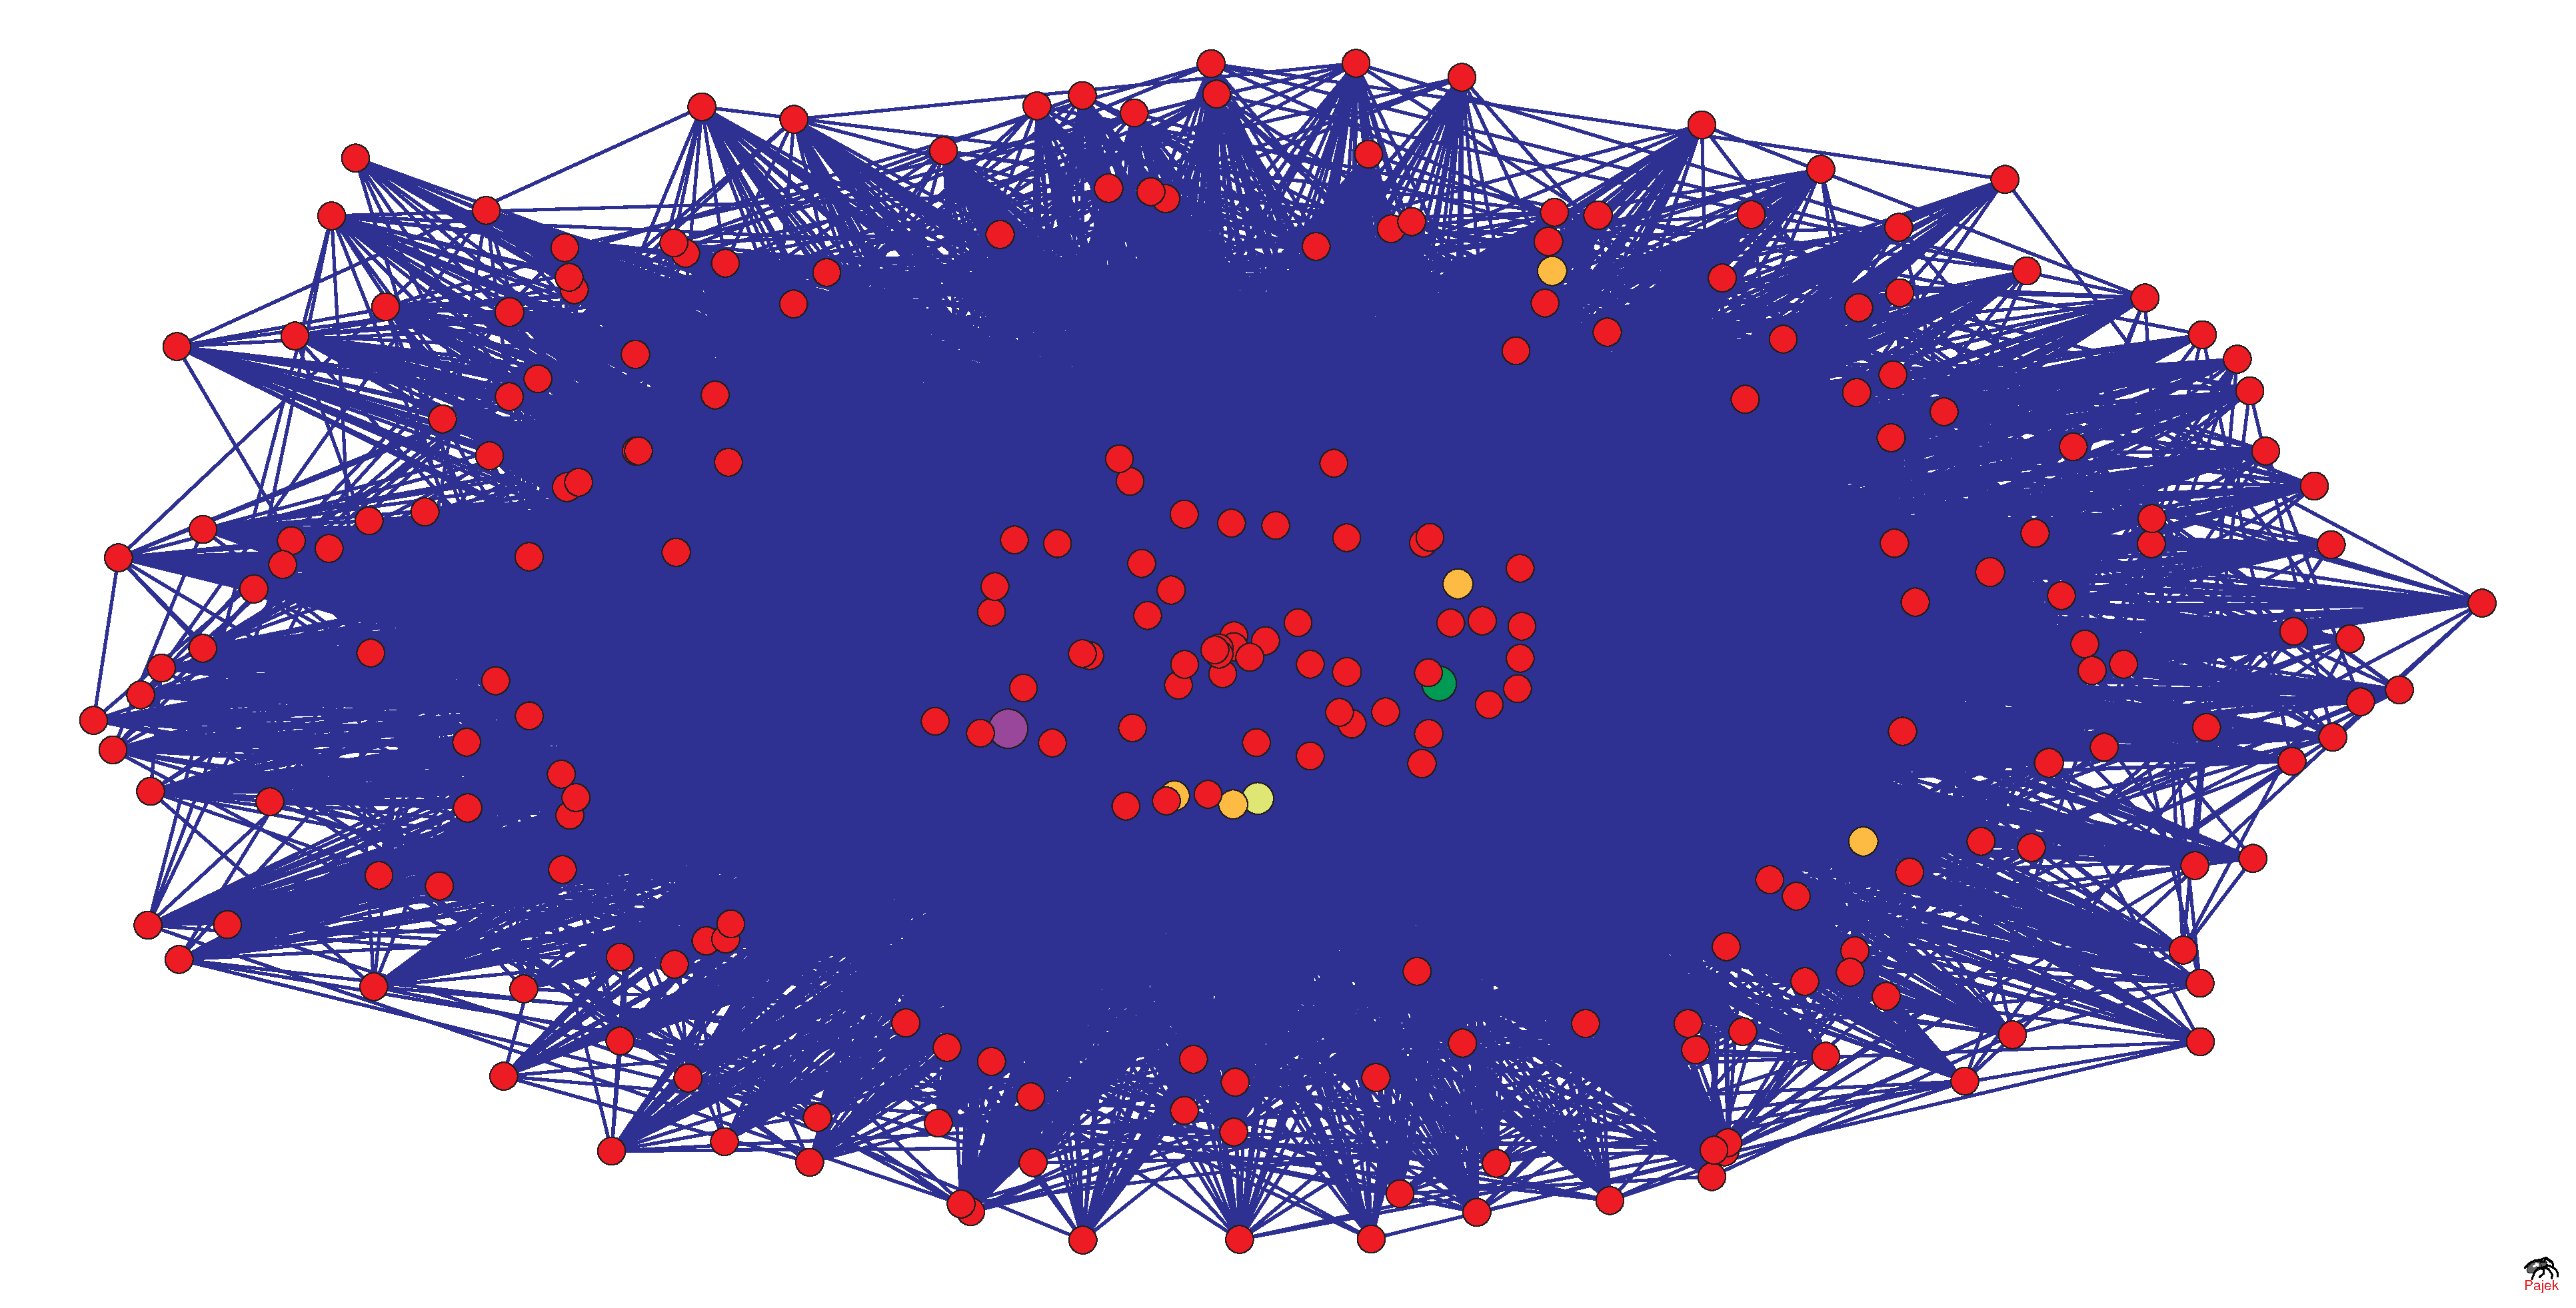
\includegraphics[width=0.76\columnwidth]{toy2_betweenness2}
\end{center}
\caption{Betweenness Centrality of "Tripartite" Graph}
\label{fig:Betweenness Centrality - Toy2}
\end{figure}
\end{frame}

\begin{frame}
\frametitle{Numerical Experiments on Synthetic Data}
\begin{figure}[h]
\begin{center}
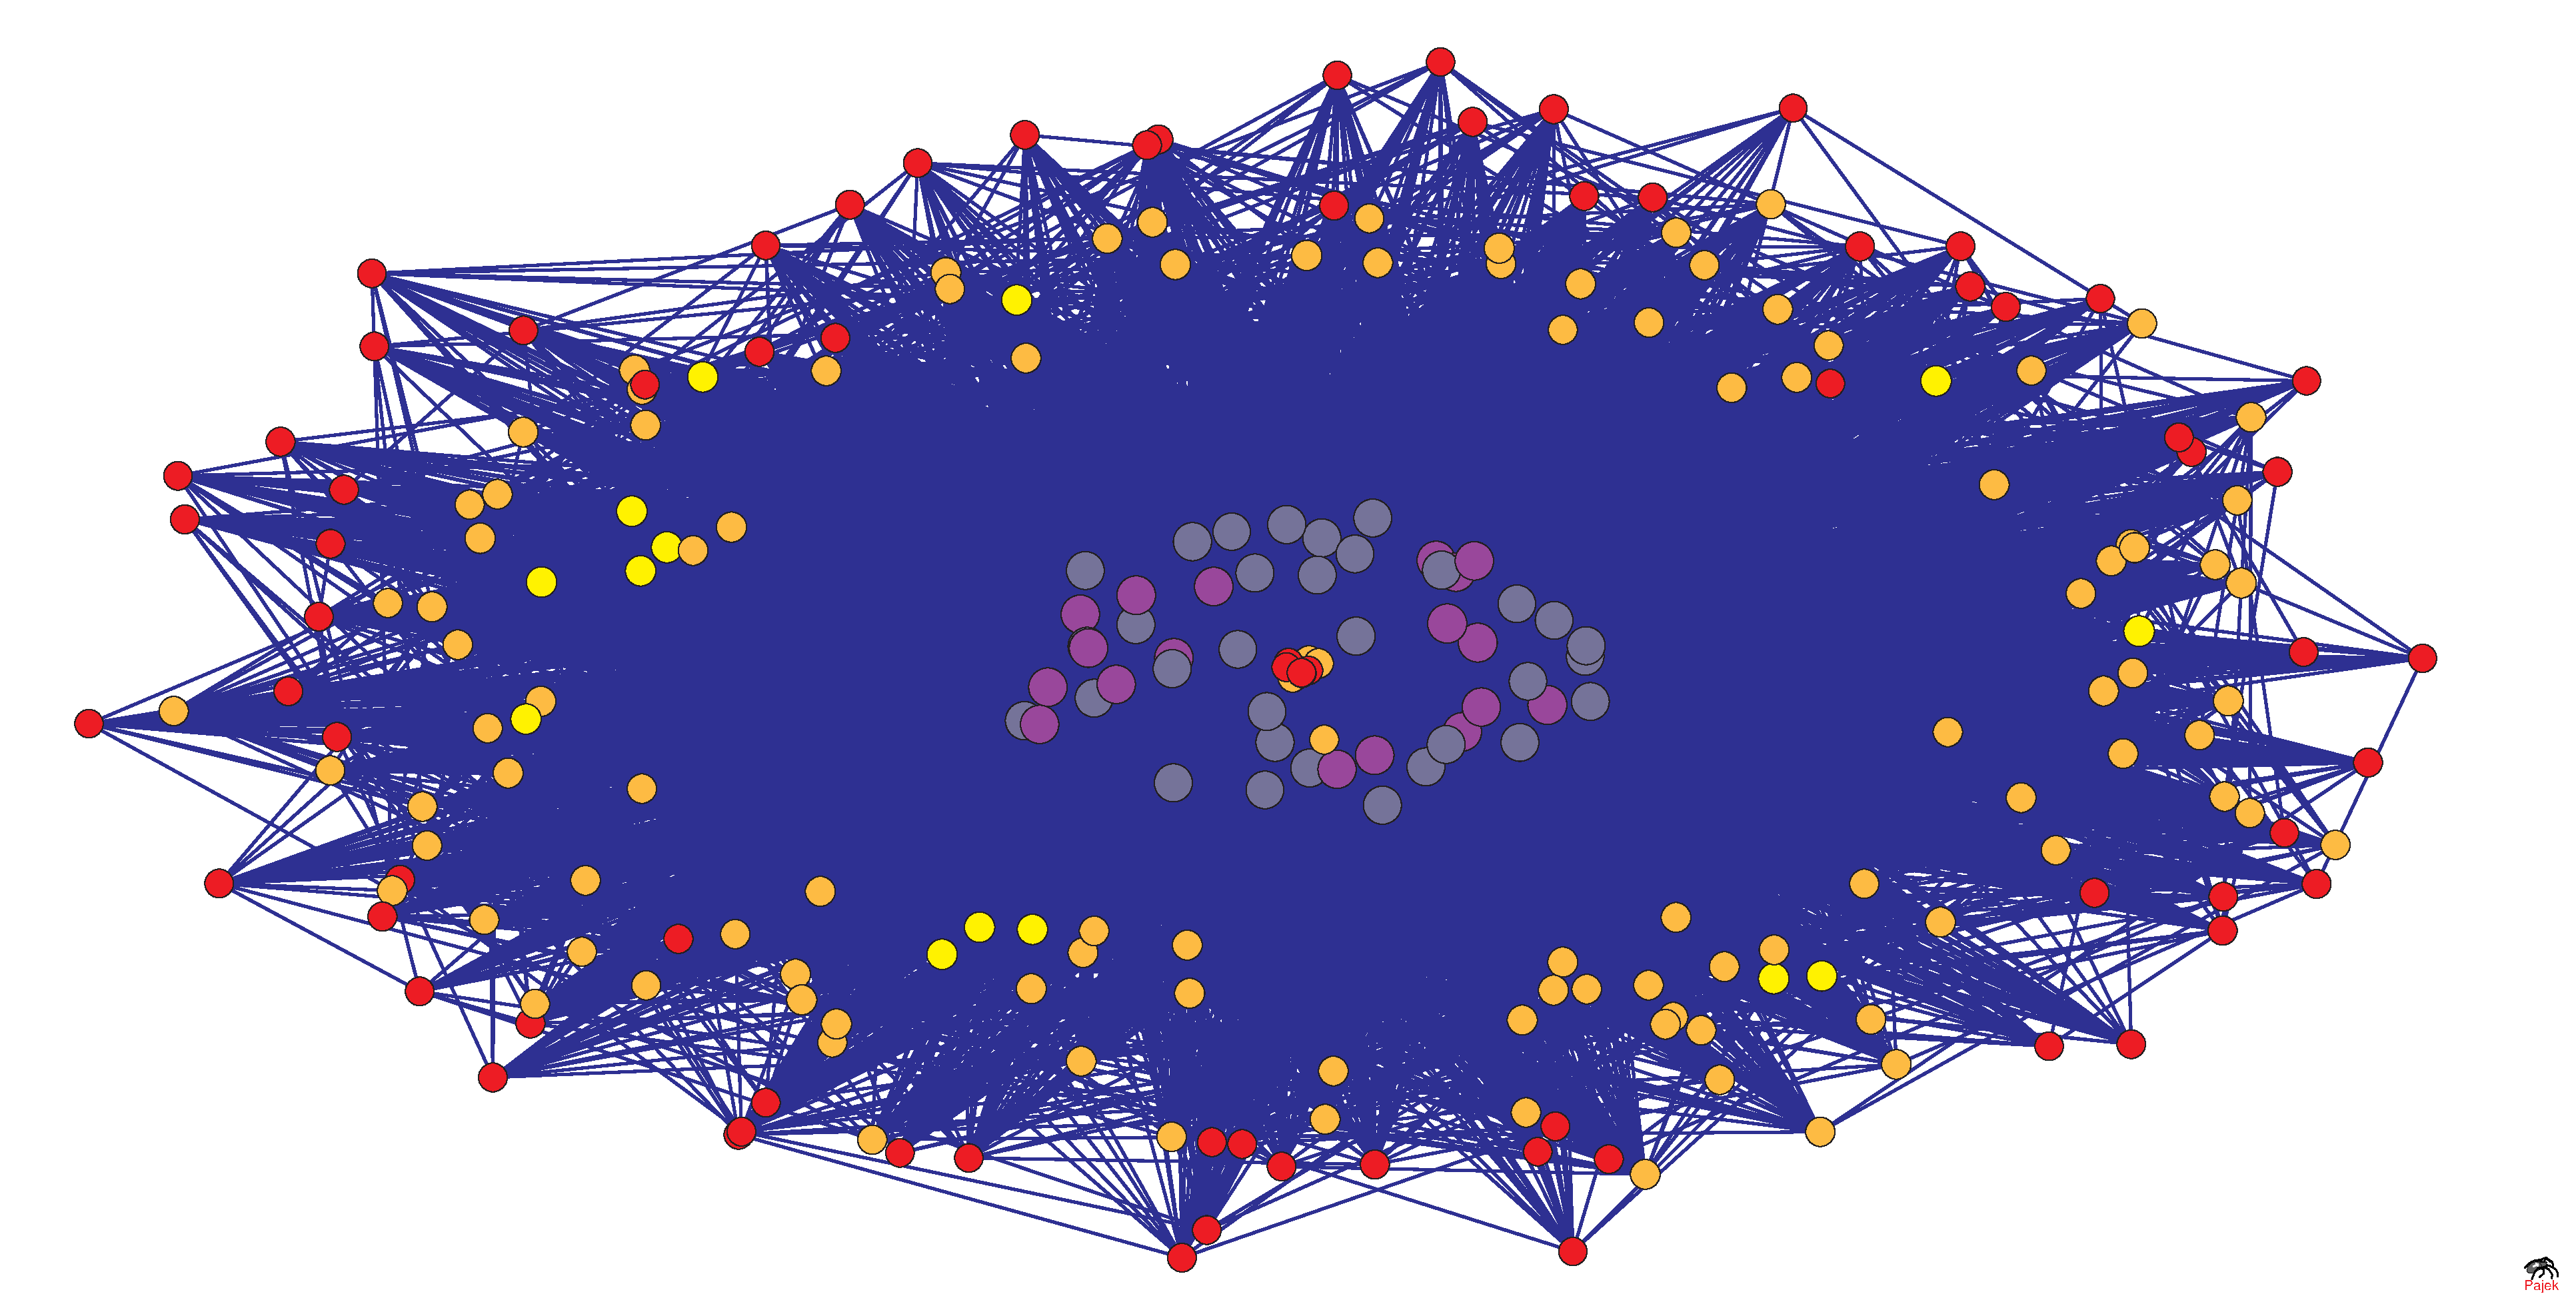
\includegraphics[width=0.76\columnwidth]{toy2_current_flow_betweenness}
\end{center}
\caption{Current-Flow Betweenness Centrality of "Tripartite" Graph}
\label{fig:Current Flow Betweenness Centrality - Toy2}
\end{figure}
\end{frame}

\begin{frame}
\frametitle{Numerical Experiments on Synthetic Data}
\begin{figure}[h]
\begin{center}
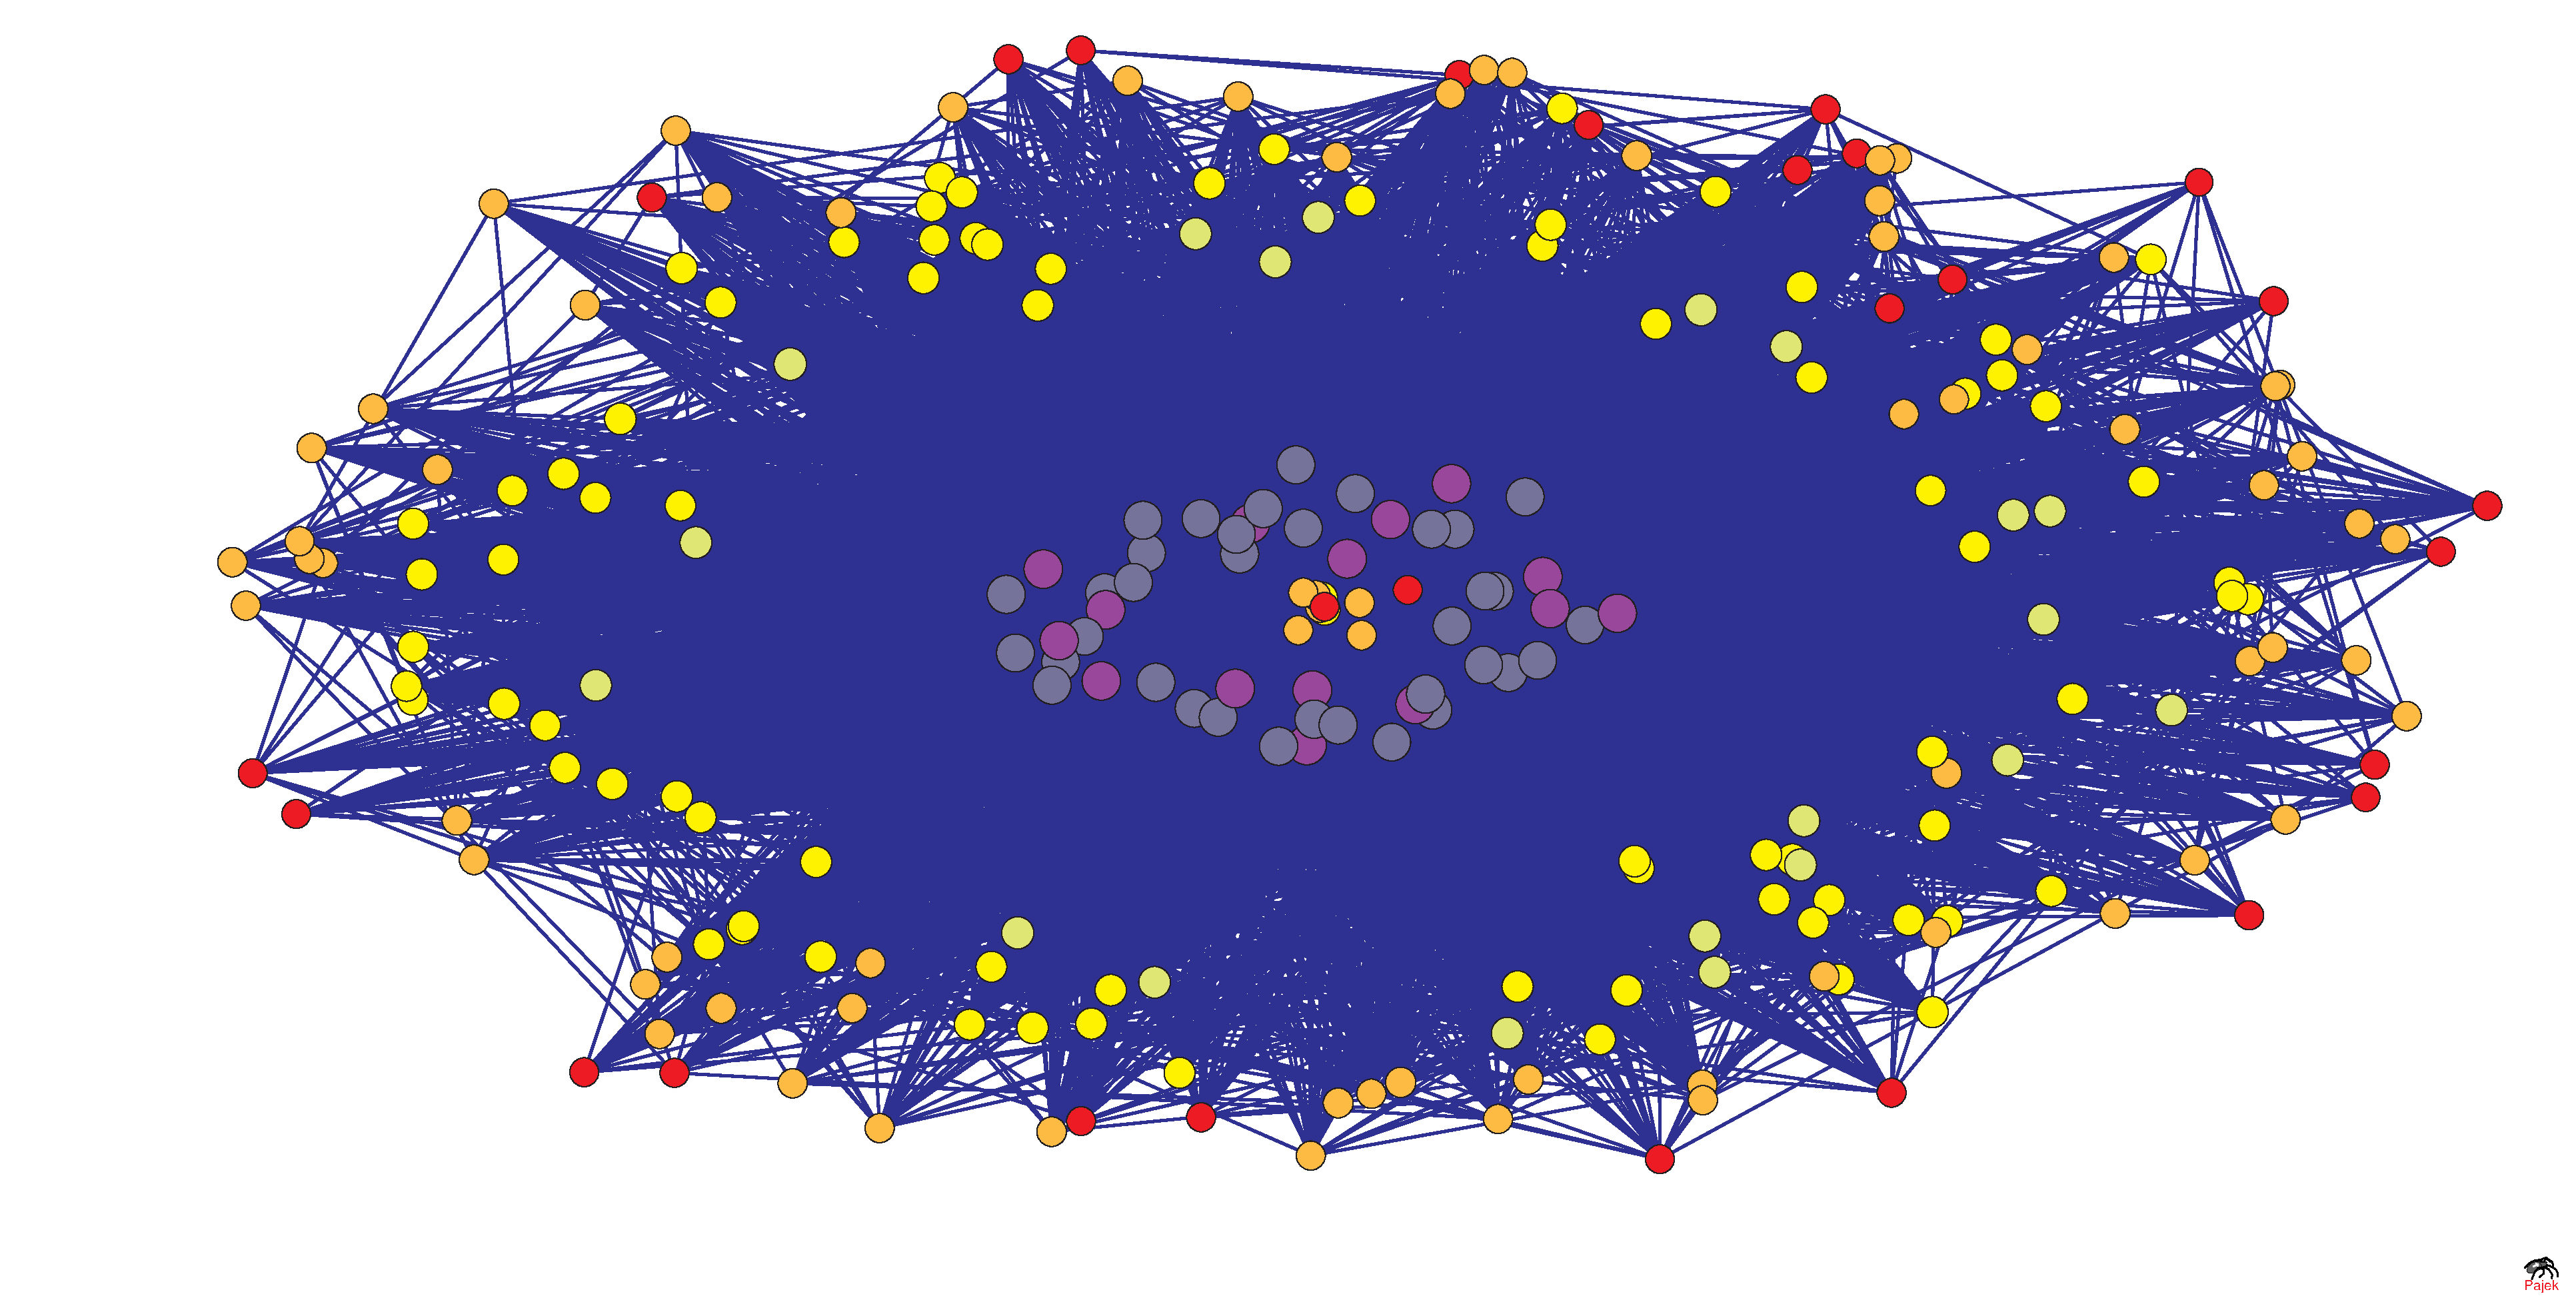
\includegraphics[width=0.76\columnwidth]{toy2_k_centrality}
\end{center}
\caption{$k$-Means Centrality of "Tripartite" Graph}
\label{fig:K-Centrality - Toy2}
\end{figure}
\end{frame}


\section{Numerical Experiments on Real Data}   \label{sec:NumExpReal}
\begin{frame}{Numerical Experiments on Real Data}
\begin{itemize}
\item We compute the centrality measures on the Florentine network, consisting of the most influential families of Florentine, Italy, during the 15th century, and the social network of Reed College. 
\begin{figure}[h]
\begin{center}
\includegraphics[width=0.50\columnwidth]{florentine.png}
\end{center}
\caption{Florentine Graph}
\label{fig:Florentine}
\end{figure}
\end{itemize}
\end{frame}

\begin{frame}
\frametitle{Numerical Experiments on Real Data}
\begin{columns}[T]
\begin{column}{.5\textwidth}
\begin{figure}[h]
\begin{center}
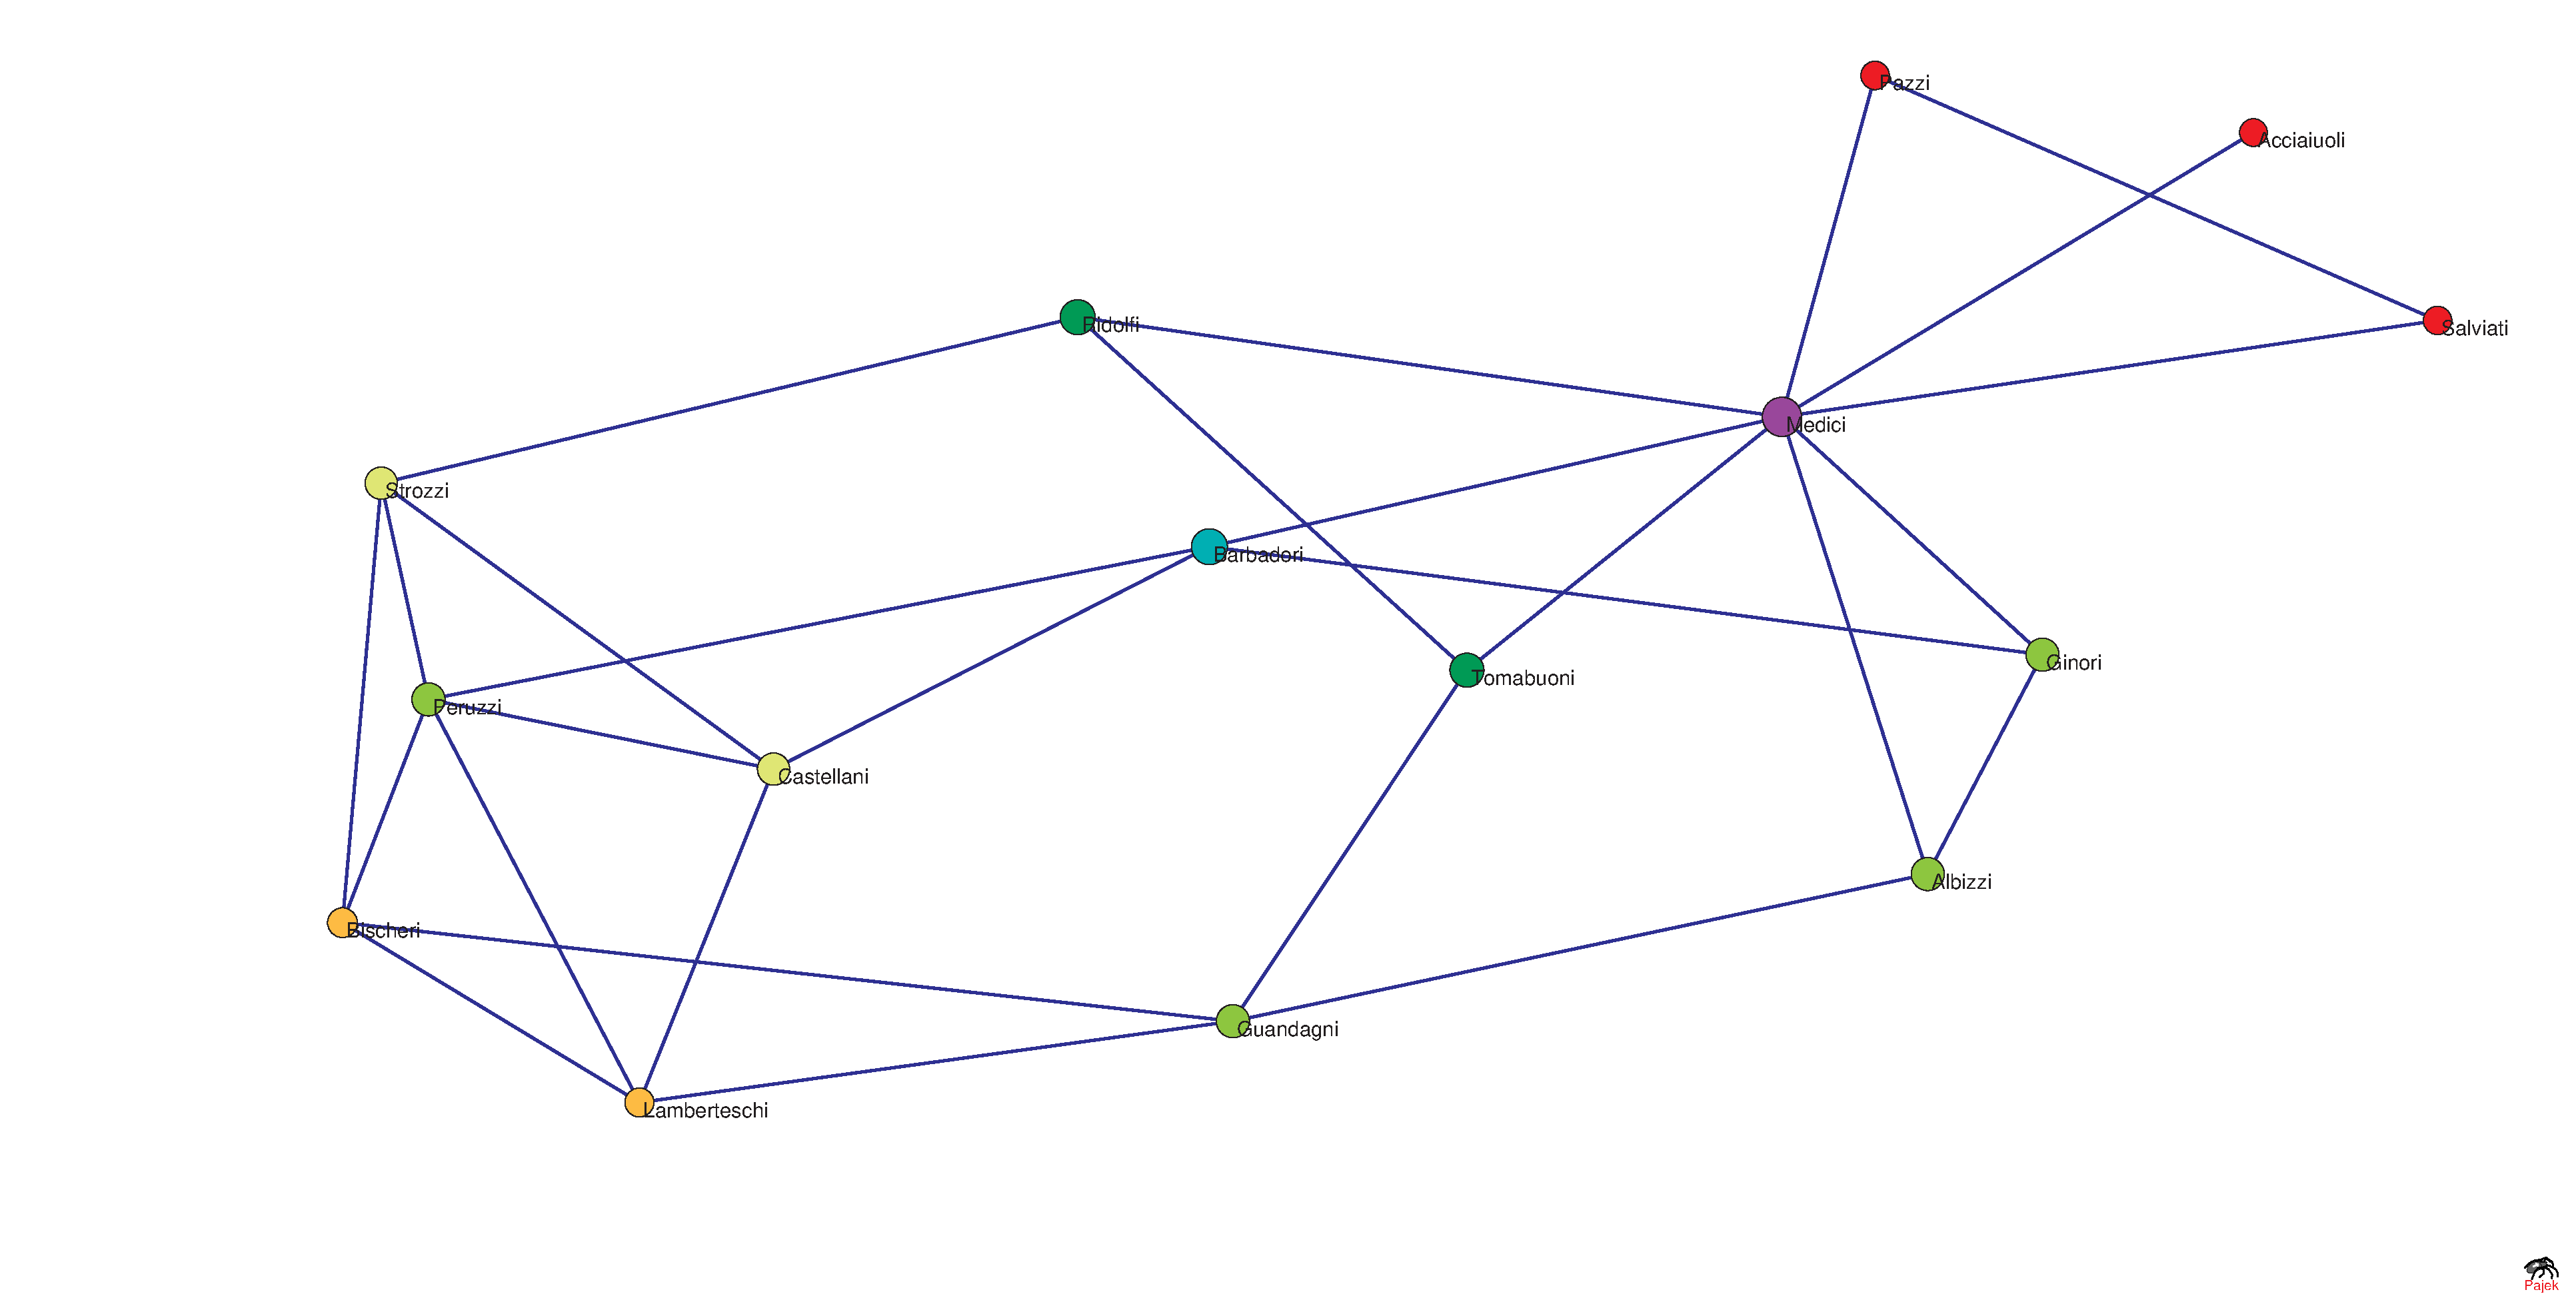
\includegraphics[width=0.76\columnwidth]{Florentine_closeness2}
\end{center}
\caption{Closeness Centrality of Florentine Network}
\label{fig:Closeness Centrality - Florentine}
\end{figure}
\end{column}
\begin{column}{.5\textwidth}
\begin{figure}[h]
\begin{center}
\includegraphics[width=0.76\columnwidth]{florentine_current_flow_closeness2}
\end{center}
\caption{Current-Flow Closeness Centrality of Florentine Network}
\label{fig:Current-Flow Closeness Centrality - Florentine}
\end{figure}
\end{column}
\end{columns}
\end{frame}

\begin{frame}
\frametitle{Numerical Experiments on Real Data}
\begin{columns}[T]
\begin{column}{.5\textwidth}
\begin{figure}[h]
\begin{center}
\includegraphics[width=0.76\columnwidth]{FlorentineBetweenness2}
\end{center}
\caption{Betweenness Centrality of Florentine Network}
\label{fig:Betweenness Centrality - Florentine}
\end{figure}
\end{column}
\begin{column}{.5\textwidth}
\begin{figure}[h]
\begin{center}
\includegraphics[width=0.76\columnwidth]{florentine_current_flow_betweenness2}
\end{center}
\caption{Current-Flow Betweenness Centrality of Florentine Network}
\label{fig:Current Flow Betweenness Centrality - Florentine}
\end{figure}
\end{column}
\end{columns}
\end{frame}

\begin{frame}
\frametitle{Numerical Experiments on Real Data}
\begin{figure}[h]
\begin{center}
\includegraphics[width=0.76\columnwidth]{FlorentineKcentrality2}
\end{center}
\caption{$k$-Means Centrality of Florentine Network}
\label{fig:K-Centrality - Florentine}
\end{figure}
\end{frame}

\begin{frame}
\frametitle{Numerical Experiments on Real Data}
\begin{figure}[h]
\begin{center}
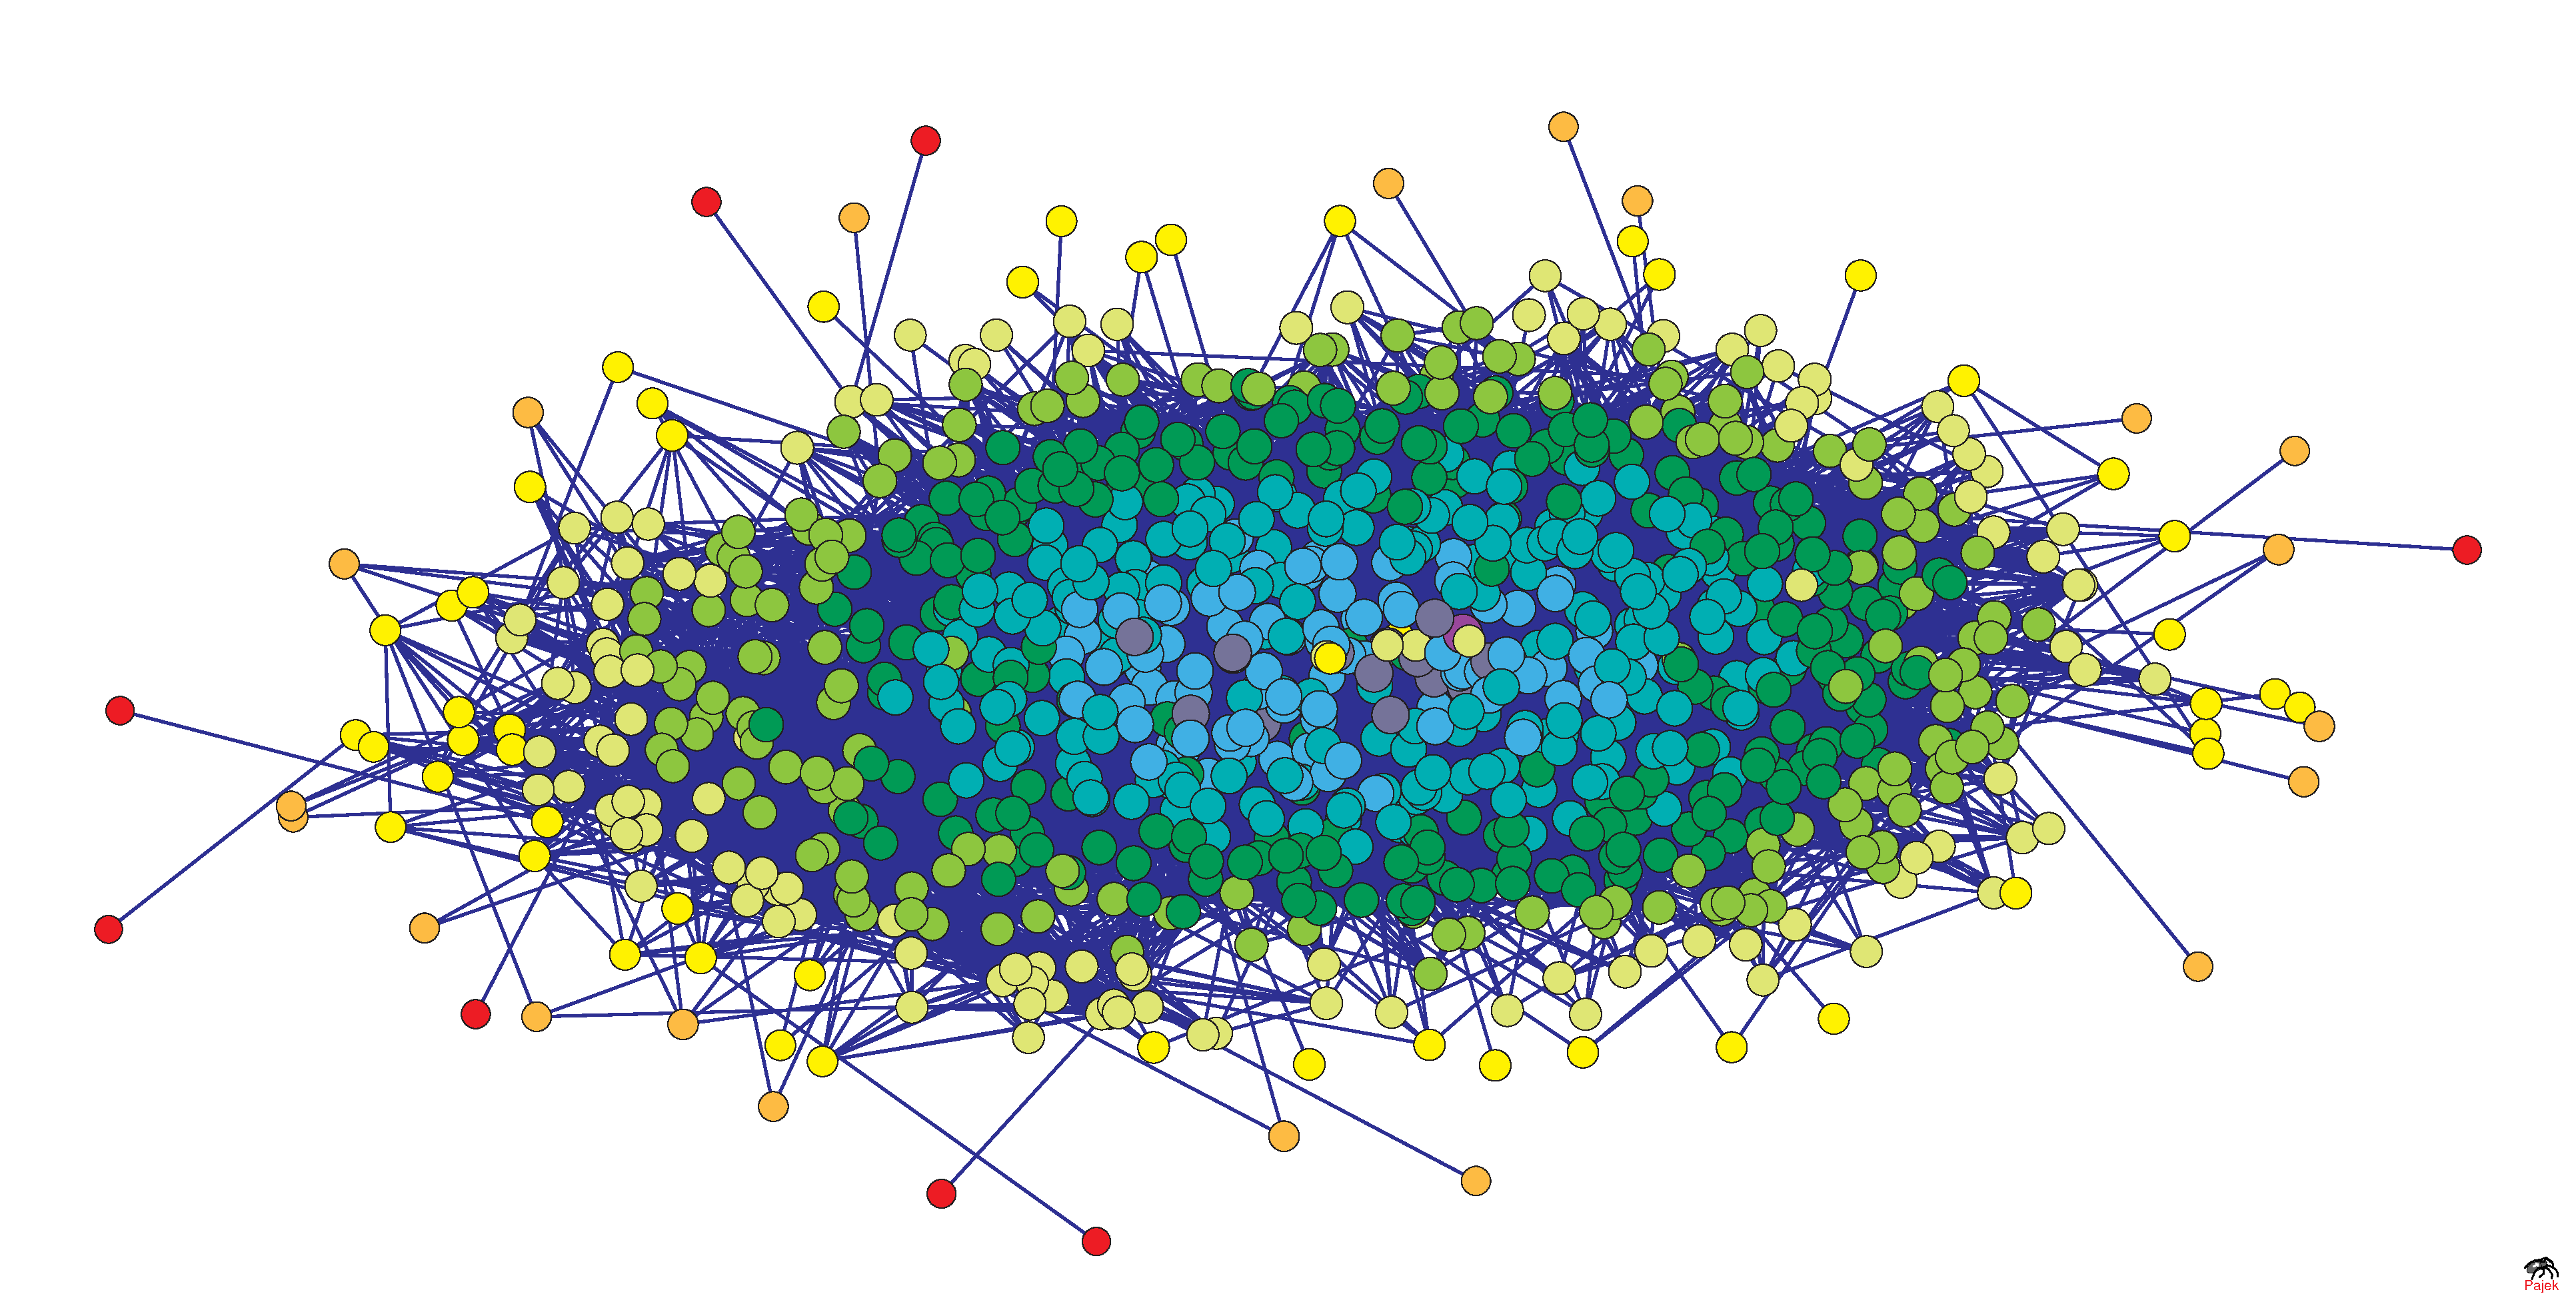
\includegraphics[width=0.76\columnwidth]{reed_closeness}
\end{center}
\caption{Closeness Centrality of Reed Network}
\label{fig:Closeness Centrality - Reed}
\end{figure}
\end{frame}


\begin{frame}
\frametitle{Numerical Experiments on Real Data}
\begin{figure}[h]
\begin{center}
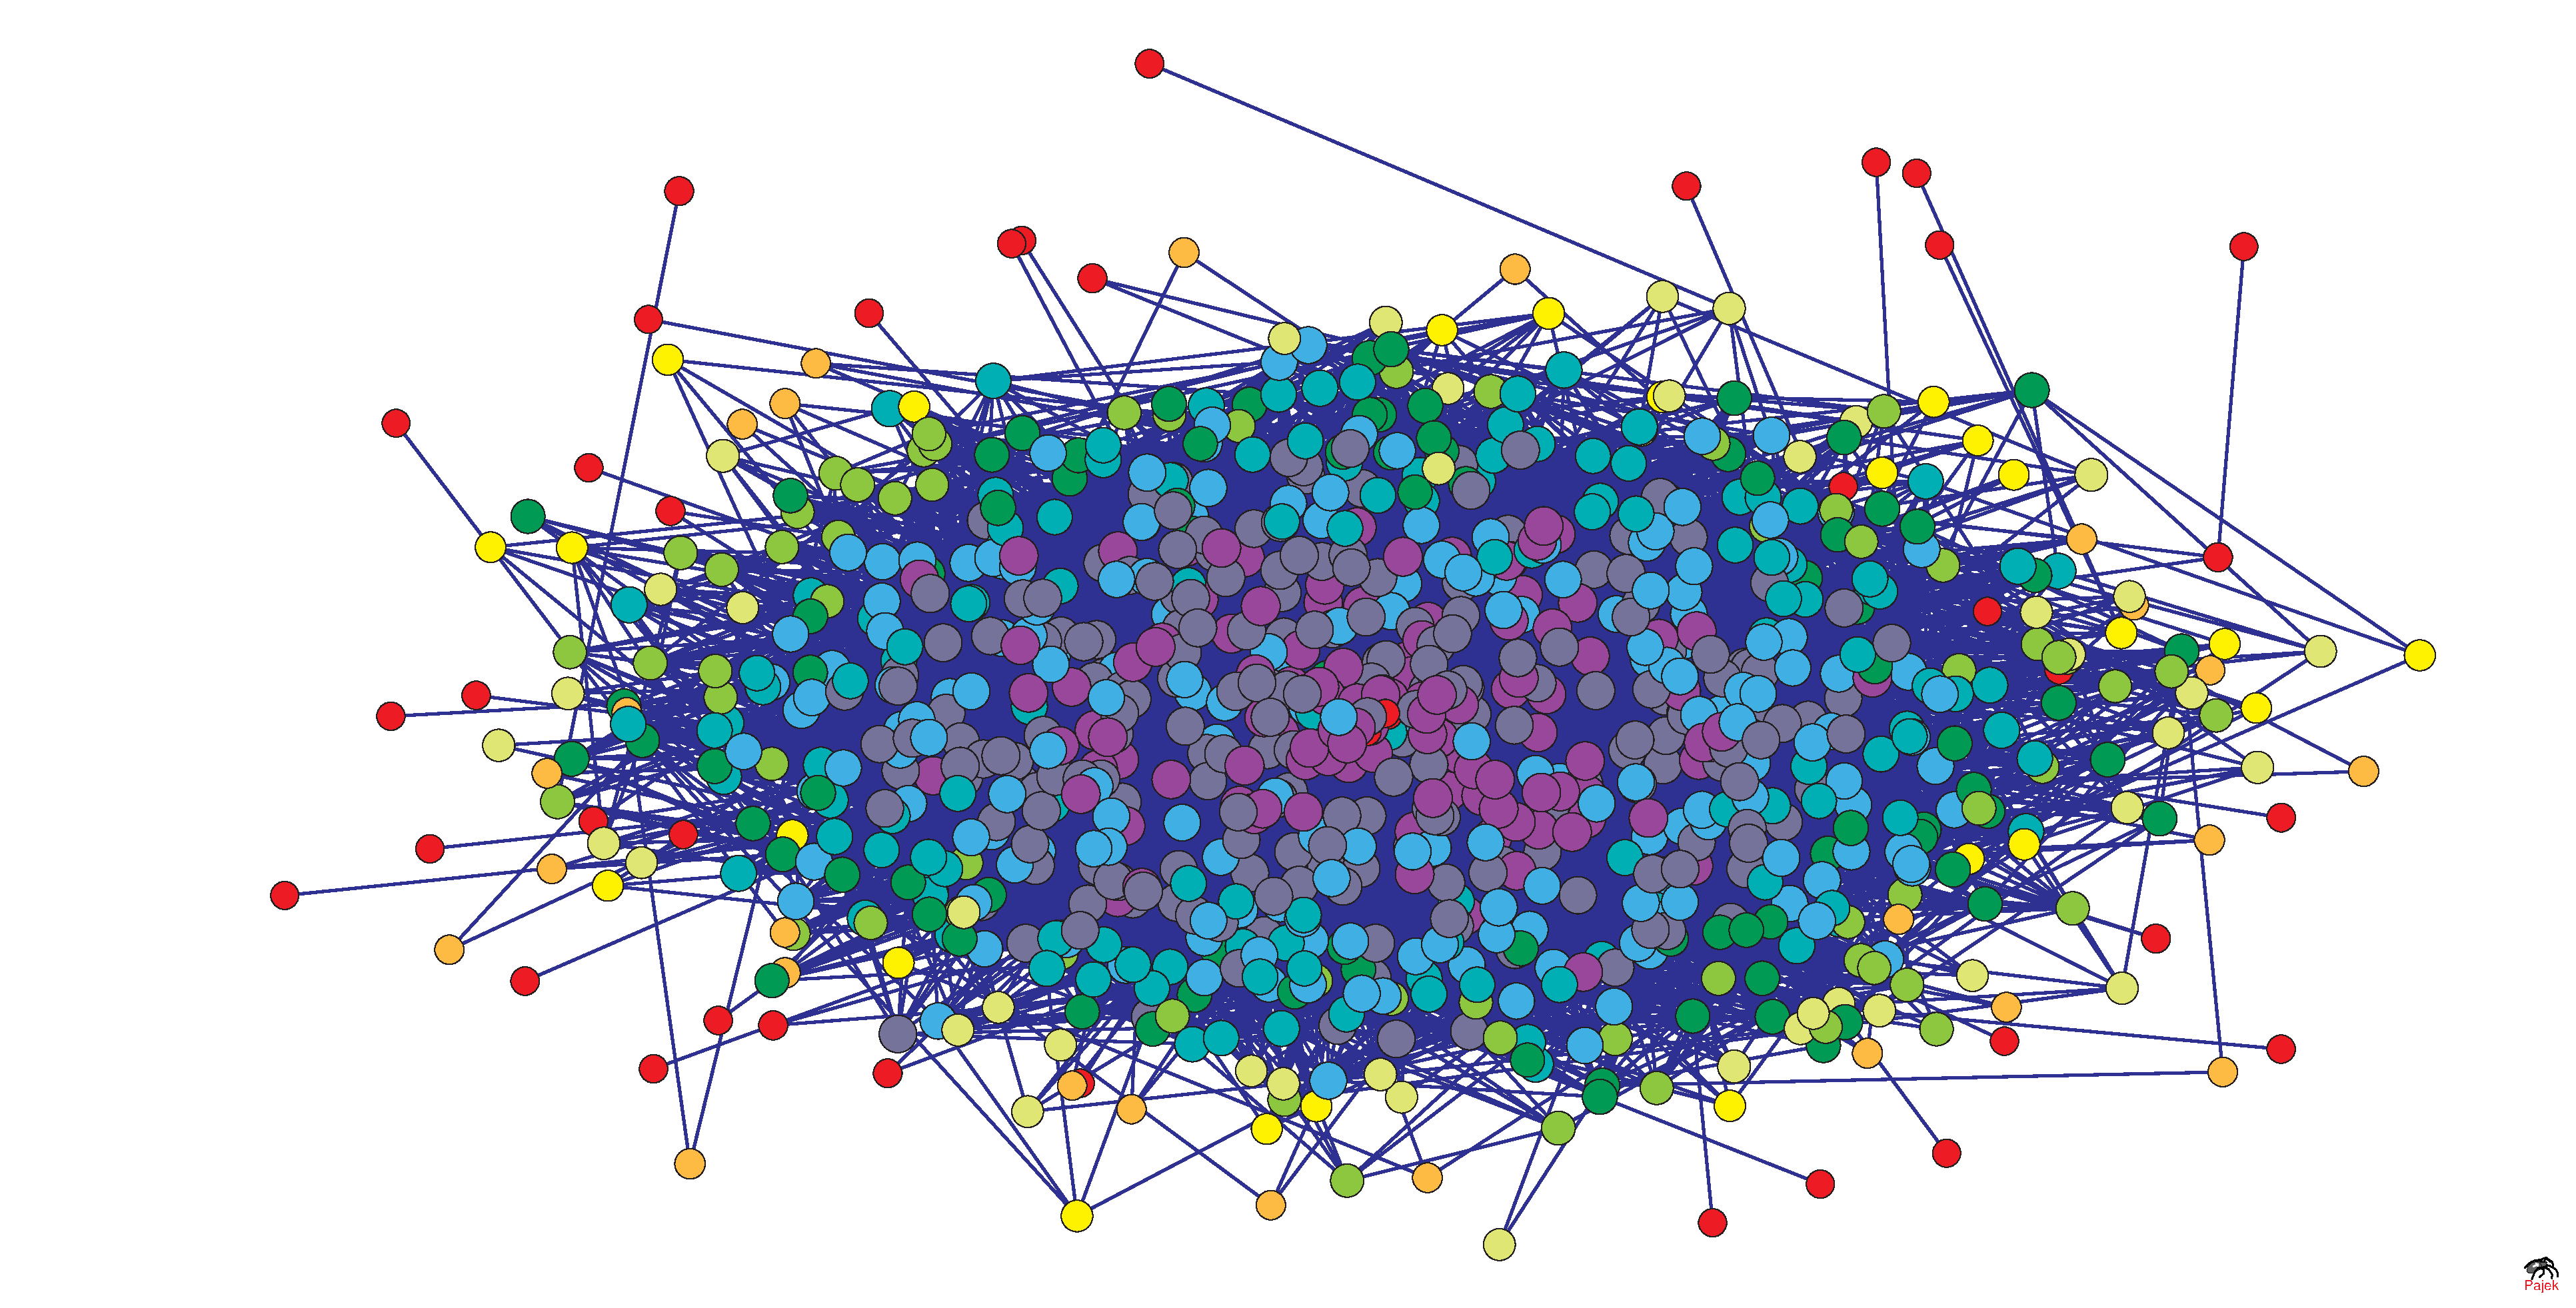
\includegraphics[width=0.76\columnwidth]{reed_current_flow_closeness}
\end{center}
\caption{Current-Flow Closeness Centrality of Reed Network}
\label{fig:Current Flow Closeness Centrality - Reed}
\end{figure}
\end{frame}

\begin{frame}
\frametitle{Numerical Experiments on Real Data}
\begin{figure}[h]
\begin{center}
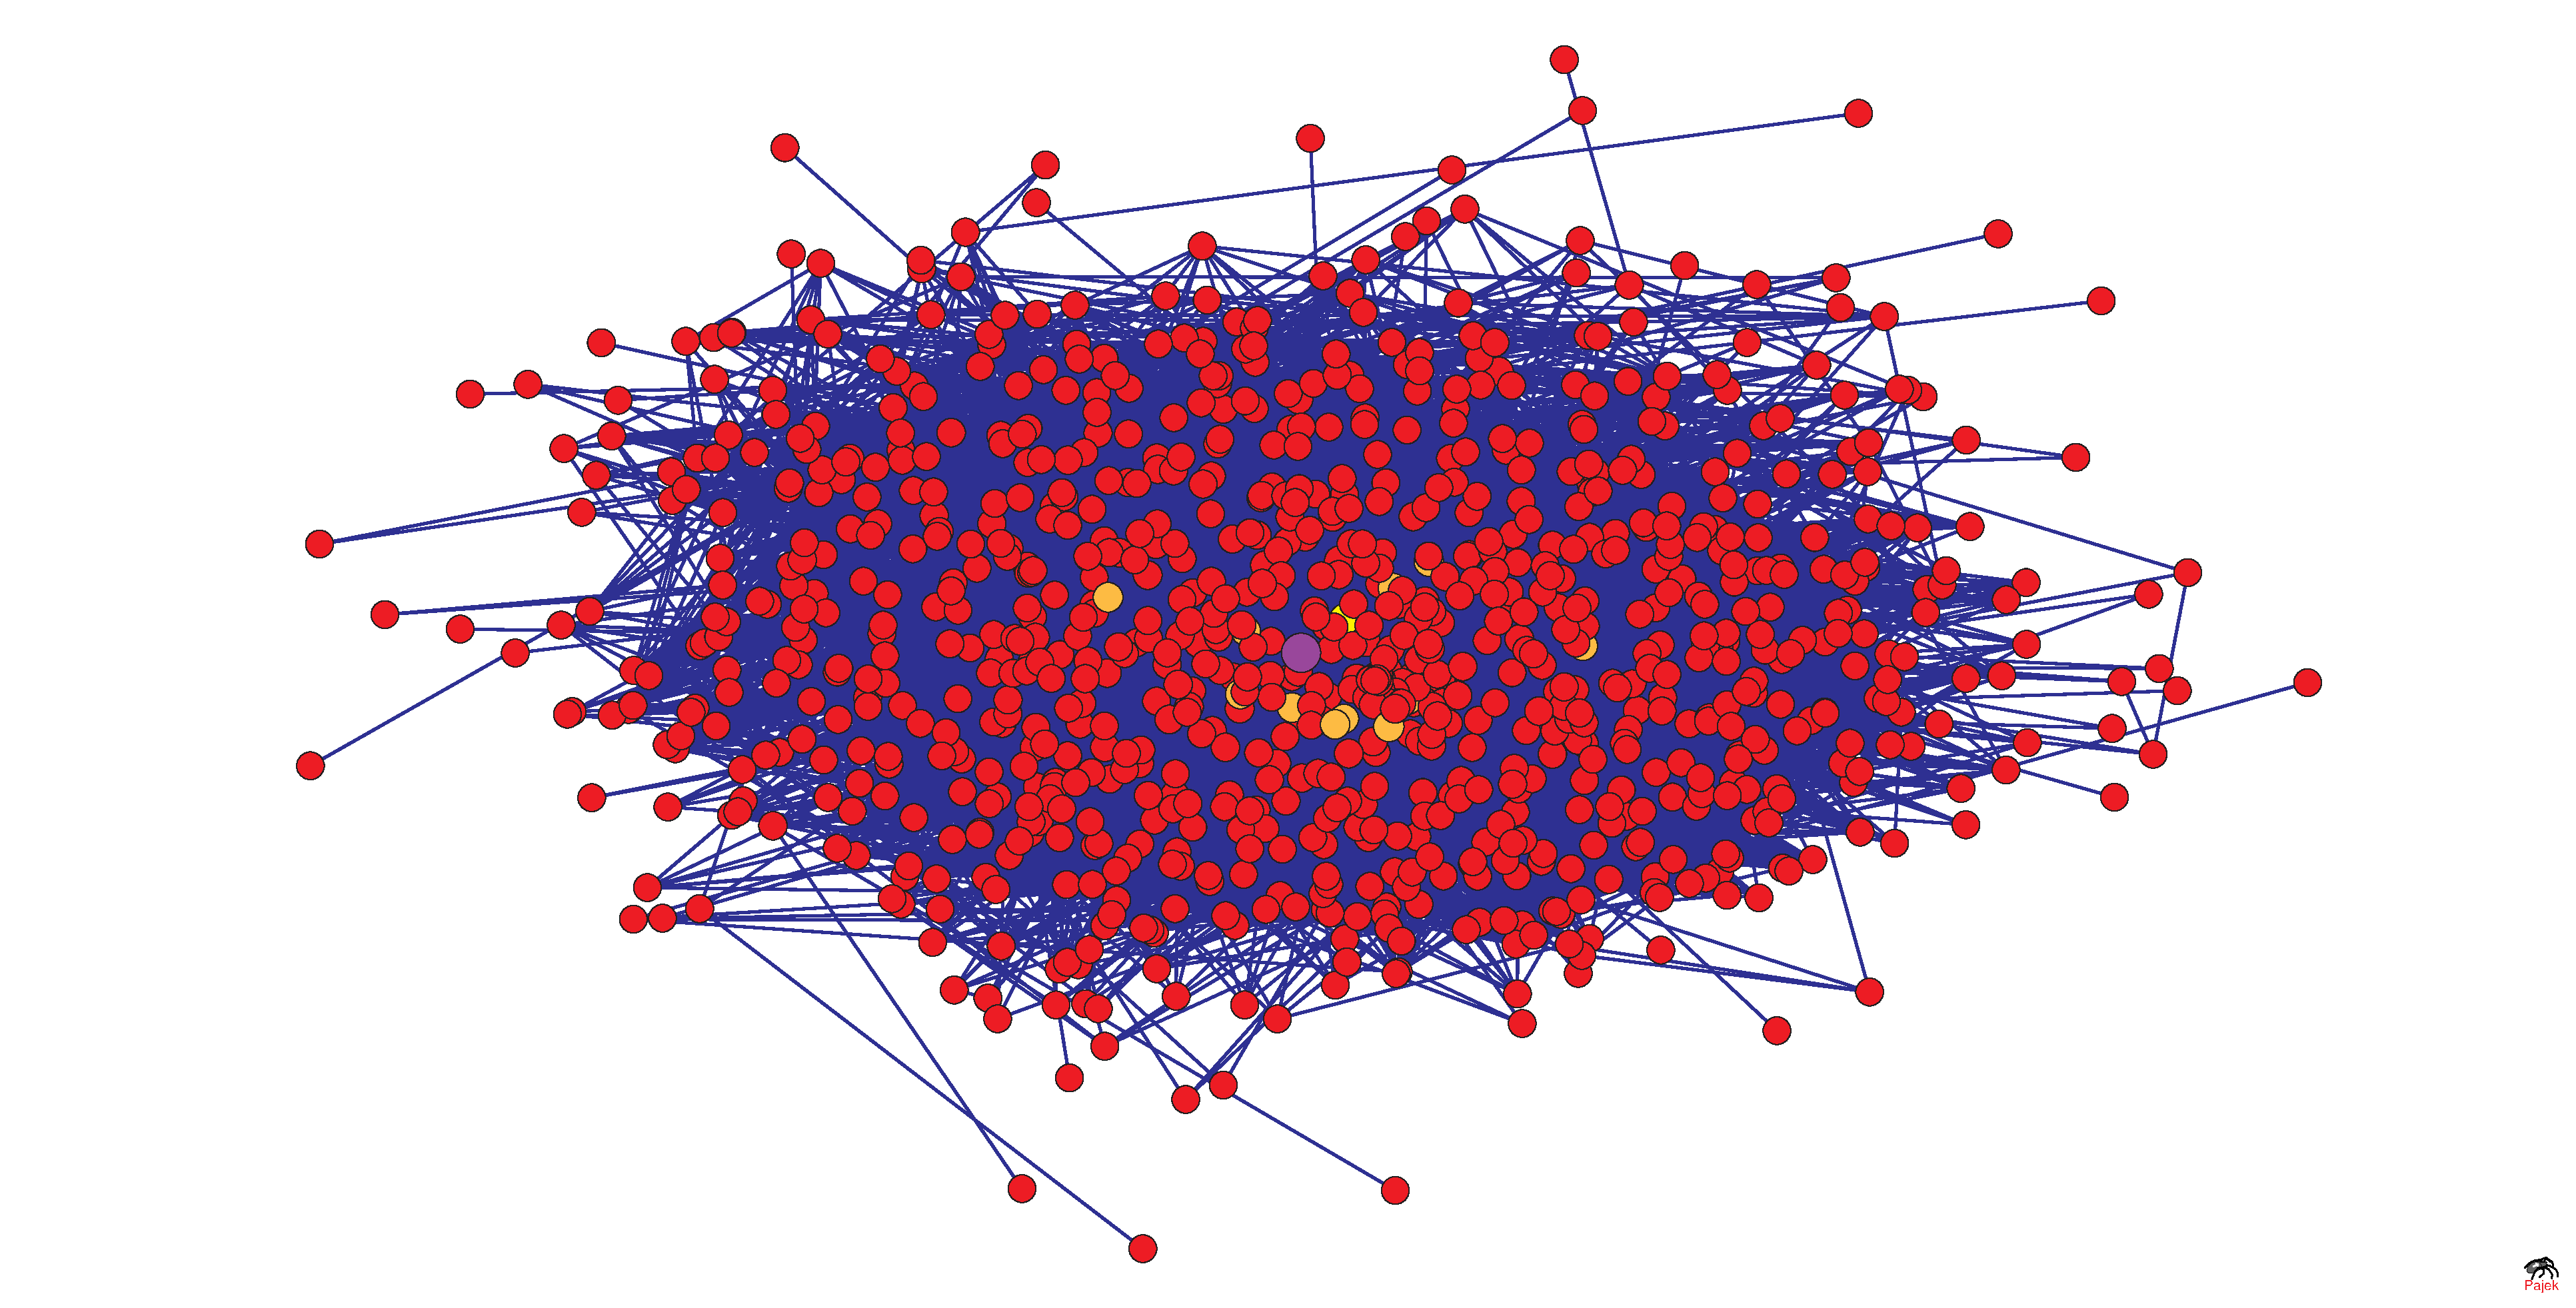
\includegraphics[width=0.76\columnwidth]{reed_betweenness}
\end{center}
\caption{Betweenness Centrality of Reed Network}
\label{fig:Betweenness Centrality - Reed}
\end{figure}
\end{frame}

\begin{frame}
\frametitle{Numerical Experiments on Real Data}
\begin{figure}[h]
\begin{center}
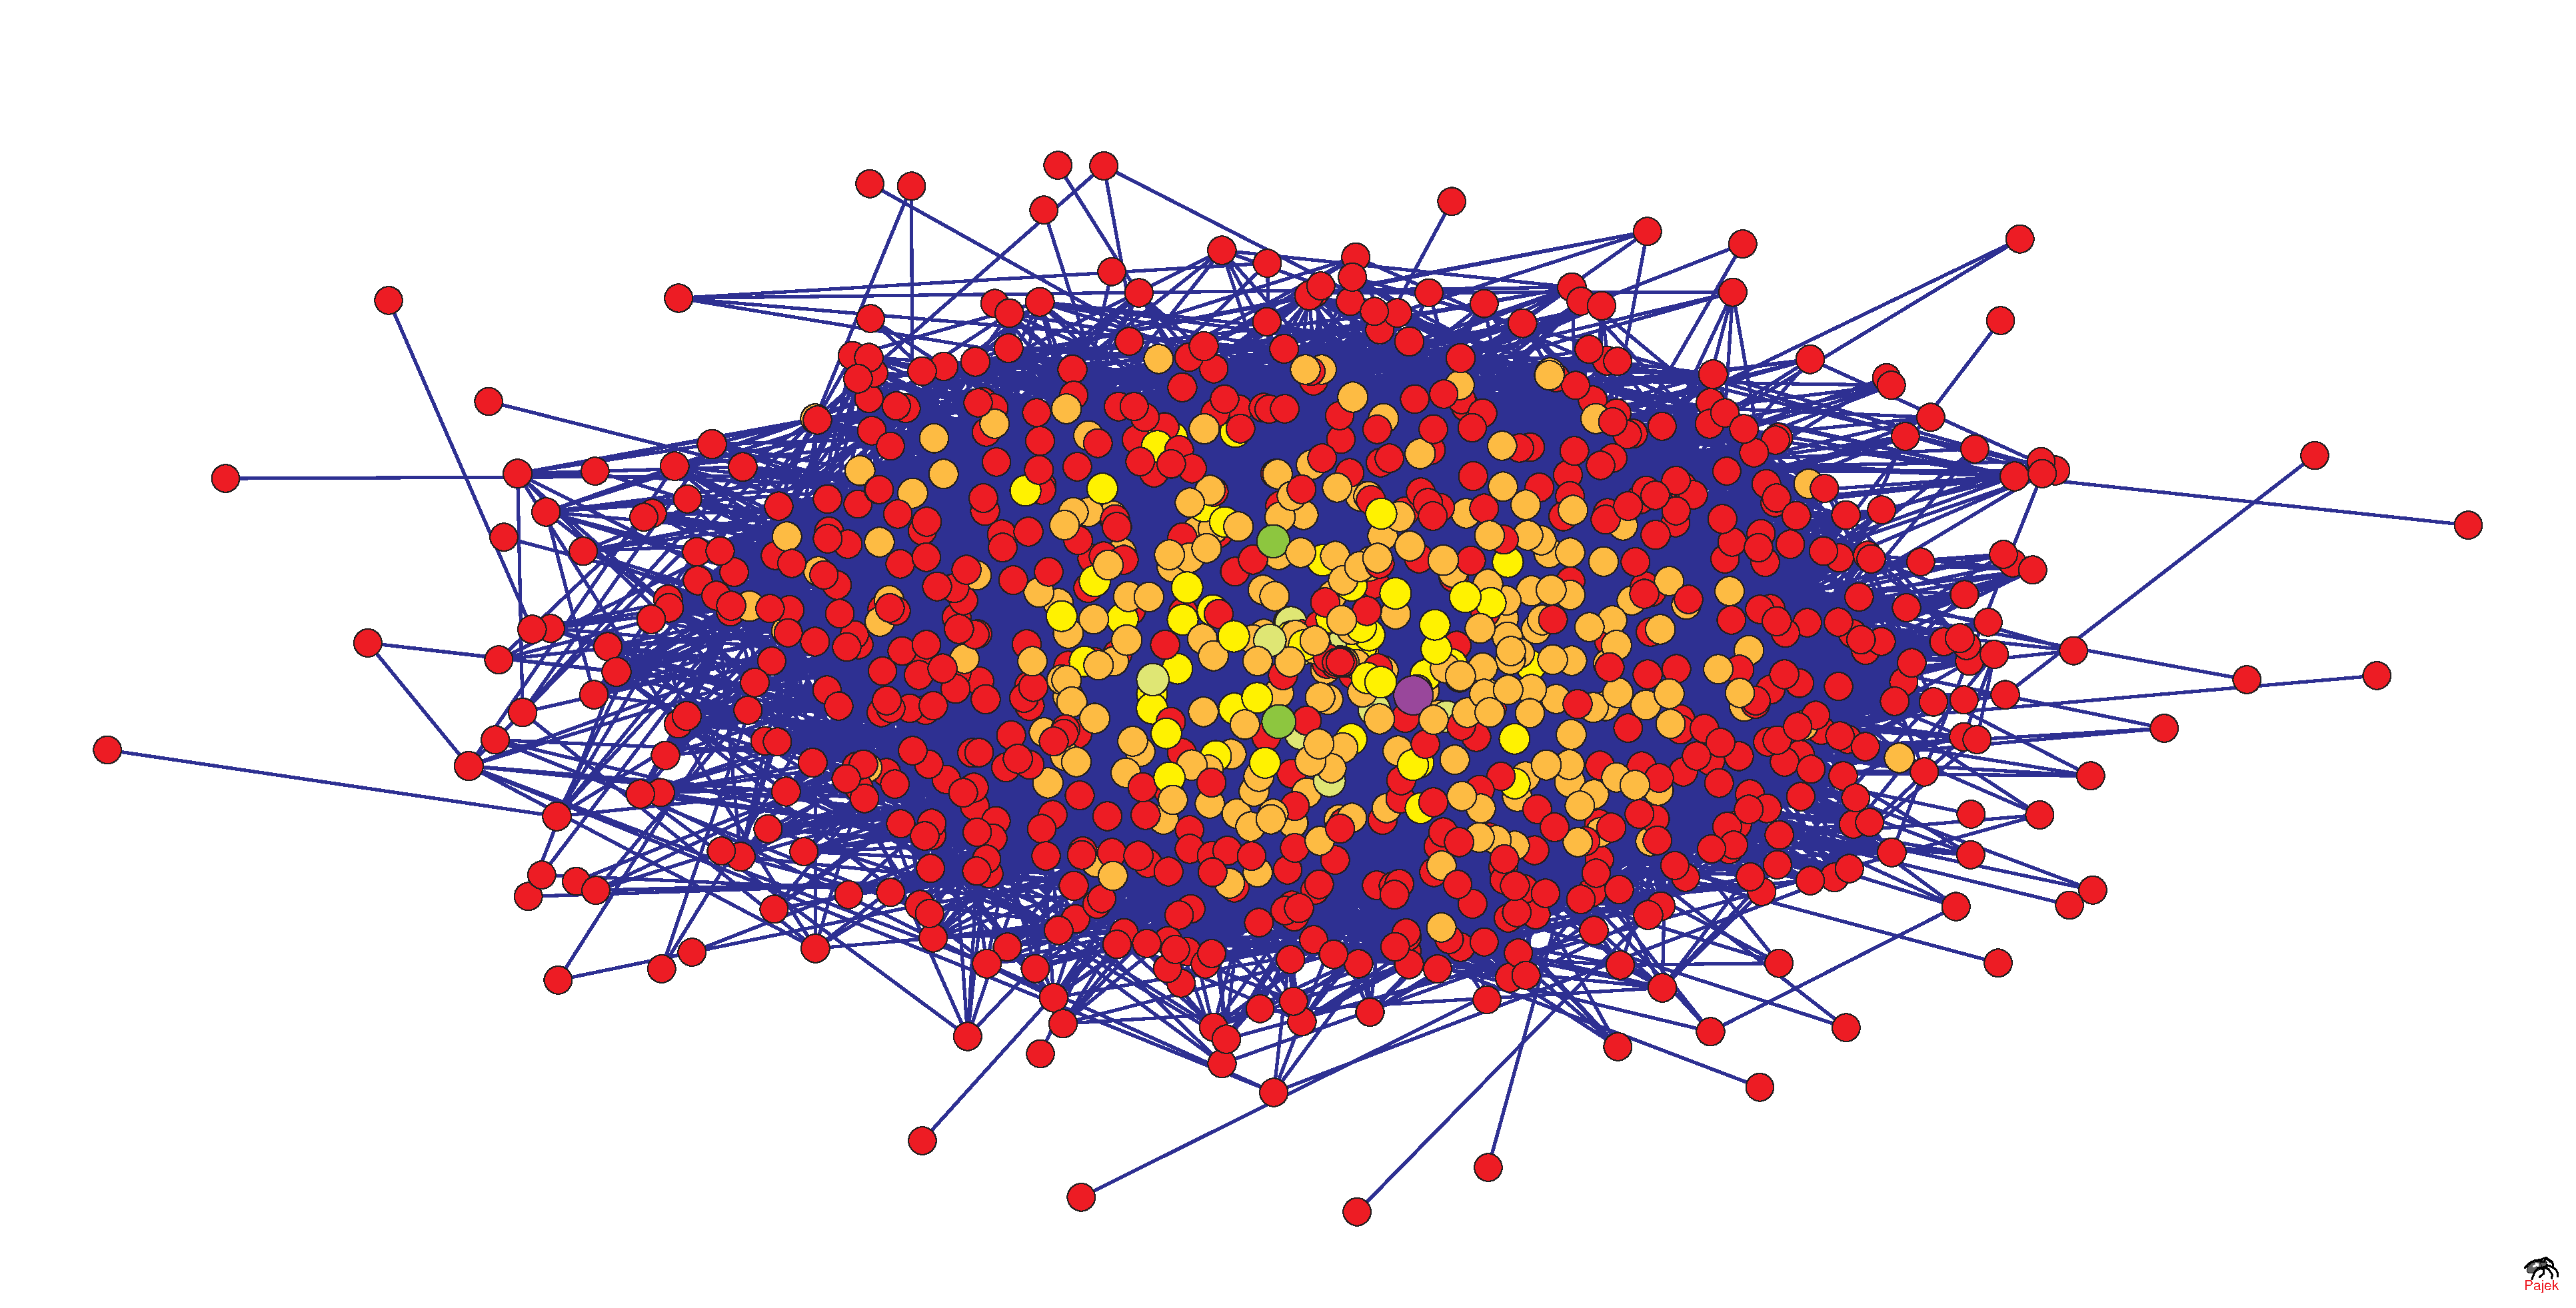
\includegraphics[width=0.76\columnwidth]{reed_current_flow_betweenness}
\end{center}
\caption{Current-Flow Betweenness Centrality of Reed Network}
\label{fig:Current Flow Betweenness Centrality - Reed}
\end{figure}
\end{frame}

\begin{frame}
\frametitle{Numerical Experiments on Real Data}
\begin{figure}[h]
\begin{center}
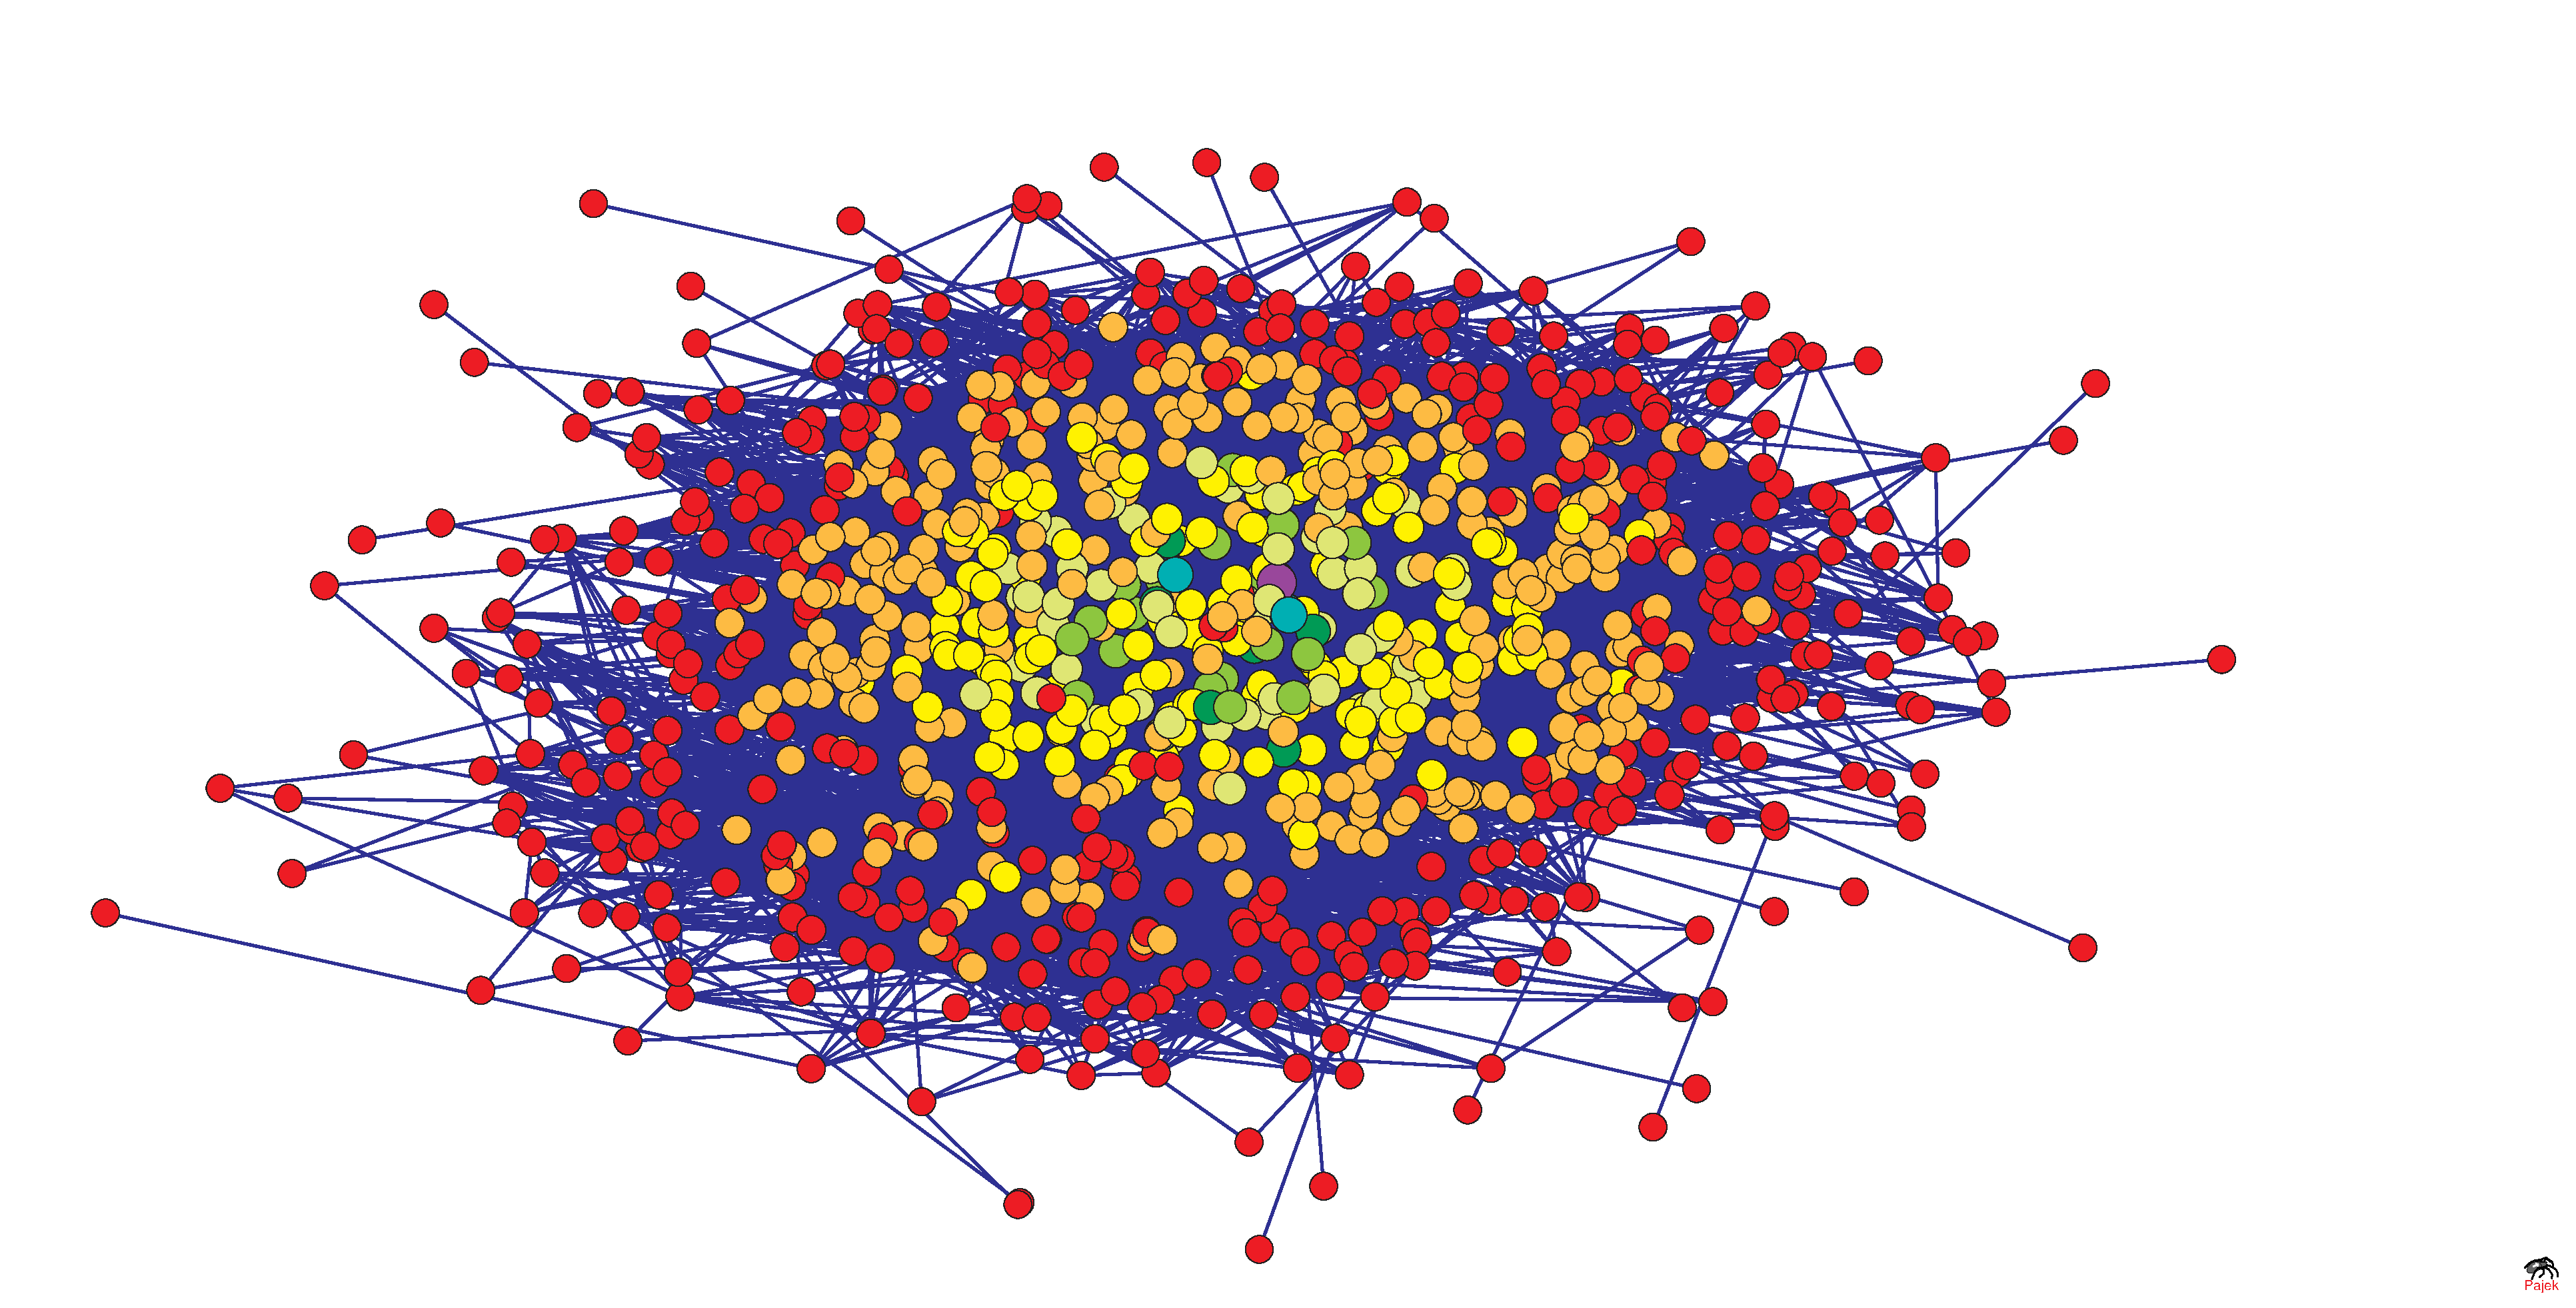
\includegraphics[width=0.76\columnwidth]{reed_k_centrality}
\end{center}
\caption{$k$-Means Centrality of Reed Network}
\label{fig:K-Centrality - Reed}
\end{figure}
\end{frame}




\section{Analysis}

\begin{frame}
     \frametitle{Discriminative Measure}
We assign a discriminative measure $\delta$ to each centrality measure:
\begin{align*}
      \delta=\sum_{i=1}^n \left[ \frac{v}{\parallel v\parallel} \right]_i,   \qquad where \quad v = \frac {\mathbb{D} \cdot \mathds{1}}{n}
     \end{align*}
$\mathbb{D}$ is the distance matrix whose $ij$-entry is the Euclidean norm of the centrality measures of the pair of nodes $i$ and $j$.\\
\vspace{5mm}

Larger discrimination measure better distinguishes different node properties

\end{frame}





\begin{frame}
\frametitle{Comparison of Discriminative Measure}
\begin{columns}[T]
\begin{column}{.5\textwidth}
\begin{figure}[h]
\begin{center}
\includegraphics[width=0.76\columnwidth]{discriminative_Florentine}
\end{center}
\caption{Discriminative Measures of Florentine Families Network}
\label{fig:Discriminative measure - Florentine}
\end{figure}
\end{column}
\begin{column}{.5\textwidth}
\begin{figure}[h]
\begin{center}
\includegraphics[width=0.76\columnwidth]{discriminative_Reed}
\end{center}
\caption{Discriminative Measures of Reed Facebook Network}
\label{fig:Discriminative measure - Reed}
\end{figure}
\end{column}
\end{columns}
\end{frame}



\begin{frame}
\frametitle{Correlation Between Centrality Measures and Node Degree}
\begin{columns}[T]
\begin{column}{.5\textwidth}
\begin{figure}[h]
\begin{center}
\includegraphics[width=0.76\columnwidth]{correlation_Florentine}
\end{center}
\caption{Correlation for Florentine Families Network}
\label{fig:Correlation  - Florentine}
\end{figure}
\end{column}
\begin{column}{.5\textwidth}
\begin{figure}[h]
\begin{center}
\includegraphics[width=0.76\columnwidth]{correlation_Reed}
\end{center}
\caption{Correlation for Reed Facebook Network}
\label{fig:Correlation - Reed}
\end{figure}
\end{column}
\end{columns}
\end{frame}


\begin{frame}
     \frametitle{Two-Cluster Separation for the "Tripartite" Graph}
We analyze how effective each measures are by trying to recover two clusters from the "tripartite" graph.
\begin{figure}
\centering
\includegraphics[width = .40\columnwidth]{twocluster.png}
\caption{Two Clusters of the "Tripartite Graph"}
\label{fig:my_label}
\end{figure}
We have 200 nodes in blue and 50 nodes in red. We also added some noise, that is some edges between the two separate blue groups. $k$-means is applied to partition the vector of centrality measures into two clusters.
\end{frame}





\begin{frame}
\frametitle{Partitioning on Closeness and Betweenness Centralities}
\begin{columns}[T]
\begin{column}{.5\textwidth}
\begin{figure}[h]
\begin{center}
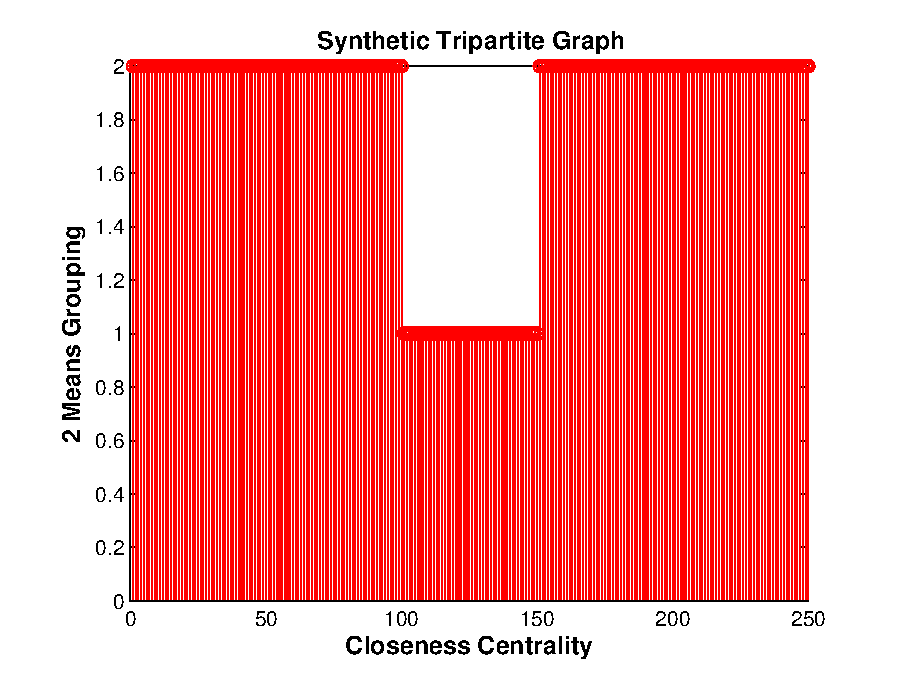
\includegraphics[width=0.76\columnwidth]{close_kmeans}
\end{center}
\caption{Closeness Centrality Partitioned into 2 Clusters}
\label{fig:closeness and k-means}
\end{figure}
\end{column}
\begin{column}{.5\textwidth}
\begin{figure}[h]
\begin{center}
\includegraphics[width=0.76\columnwidth]{betw_kmeans}
\end{center}
\caption{Betweenness Centrality Partitioned into 2 Clusters}
\label{fig:betweenness and k-means}
\end{figure}
\end{column}
\end{columns}
\end{frame}

\begin{frame}
\frametitle{Partitioning on Current-Flow Closeness and Current-Flow Betweenness Centralities}
\begin{columns}[T]
\begin{column}{.5\textwidth}
\begin{figure}[h]
\begin{center}
\includegraphics[width=0.76\columnwidth]{cfclose_kmeans}
\end{center}
\caption{Current-Flow Closeness Centrality Partitioned into 2 Clusters}
\label{fig:Current Flow closeness and k-means}
\end{figure}
\end{column}
\begin{column}{.5\textwidth}
\begin{figure}[h]
\begin{center}
\includegraphics[width=0.76\columnwidth]{cfbetw_kmeans}
\end{center}
\caption{Current-Flow Betweenness Centrality Partitioned into 2 Clusters}
\label{fig:Current Flow betweenness and k-means}
\end{figure}
\end{column}
\end{columns}
\end{frame}


\begin{frame}
\frametitle{Partitioning on $k$-means Centrality}
\begin{figure}[h]
\begin{center}
\includegraphics[width=0.76\columnwidth]{kcent_kmeans}
\end{center}
\caption{$k$-means Centrality Partitioned into 2 Clusters}
\label{fig:K-mean cluster on centrality score}
\end{figure}
\end{frame}




\begin{frame}
     \frametitle{Average Distance Test on "Tripartite Graph"}
     \begin{itemize}
     \item We sort the vector of centrality measures in         descending order.
     \item We divide the vector into two groups of size $p$ and $q$ such that $p+q=n$ and compute the distance matrices $D_1$ and $D_2$ of the two groups.
     \item We plot $\lambda = \frac{\sigma_1 + \sigma_2}{2}$ for each cut point $p$ where
     \begin{align*}
      \sigma_1 = \frac{\sum_{k=1}^p [D_1 \cdot \mathds{1}]_k}{\binom{p}{2}},
      \quad
      \sigma_2 = \frac{\sum_{k=1}^q [D_2 \cdot \mathds{1}]_k}{\binom{q}{2}}
     \end{align*}
     
\item $\lambda$ is expected to obtain its minimum at $p=50$ since that is where we divide the nodes with high centrality measures and nodes with low centrality measures into their own groups.
\end{itemize}
\end{frame}




%\begin{frame}
%     \frametitle{Average Distances (continued)}
%     \vspace{1mm}
%     \begin{align*}
%      \lambda = \frac{avg1 + avg2}{2},
%      \quad
%\mathds{1}]_k}{\binom{i}{2}},
%      \quad
%      avg2 = \frac{\sum_{j=1}^n [D2 * %\mathds{1}]_j}{\binom{n-i}{2}}
%     \end{align*}
%    \begin{align*}
%      D1 = D(\gamma_1,\gamma_1),\quad
%      D2 = D(\gamma_2,\gamma_2)
%     \end{align*}
%     \begin{itemize}
%    \item Resulting average distance, $\lambda$ is the mean of the top and bottom averages
%     \item D1 is the submatrix representing the distances of the top nodes
%     \item D2 is the submatrix representing the distances of the bottom nodes
%    \item $\gamma_1$ and $\gamma_2$ are vectors of indices of the nodes in the top cut and bottom cut, respectively
%     \end{itemize}
%\end{frame}



\begin{frame}
\frametitle{Average Distance Test for Closeness and Betweenness Centralities}
\begin{columns}[T]
\begin{column}{.5\textwidth}
\begin{figure}[h]
\begin{center}
\includegraphics[width=0.80\columnwidth]{avgdist_close}
\end{center}
\caption{Average Distance for Closeness Centrality}
\label{fig:Average distance for closeness centrality vector}
\end{figure}
\end{column}
\begin{column}{.5\textwidth}
\begin{figure}[h]
\begin{center}
\includegraphics[width=0.80\columnwidth]{avgdist_betw}
\end{center}
\caption{Average Distance for Betweenness Centrality}
\label{fig:Average distance for betweenness centrality vector}
\end{figure}
\end{column}
\end{columns}
\end{frame}


\begin{frame}
\frametitle{Average Distance Test for Current-Flow Closeness and Current-Flow Betweenness Centralities}
\begin{columns}[T]
\begin{column}{.5\textwidth}
\begin{figure}[h]
\begin{center}
\includegraphics[width=0.76\columnwidth]{avgdist_cfclose}
\end{center}
\caption{Average Distance for Current-Flow Closeness}
\label{fig:Average distance for current flow closeness centrality vector}
\end{figure}
\end{column}
\begin{column}{.5\textwidth}
\begin{figure}[h]
\begin{center}
\includegraphics[width=0.76\columnwidth]{avgdist_cfbetw}
\end{center}
\caption{Average Distance for Current-Flow Betweenness}
\label{fig:Average distance for current flow betweenness centrality vector}
\end{figure}
\end{column}
\end{columns}
\end{frame}


\begin{frame}
\frametitle{Average Distance Test for $k$-Means Centrality }
\begin{figure}[h]
\begin{center}
\includegraphics[width=0.76\columnwidth]{avgdist_kcent}
\end{center}
\caption{Average Distance for $k$-means Centrality}
\label{fig:Average distance for k centrality}
\end{figure}
\end{frame}








\section{Summary and conclusion}  \label{sec:conclusion}

\begin{frame}
\frametitle{Summary of Our Work}
\begin{itemize}
\item $k$-means centrality ranks in the middle in terms of discriminative measure since it measures less than closeness and current-flow closeness but more than betweenness and current-flow betweenness.
\item $k$-means centrality has the highest correlation to node degree among the five centrality measures.
\item Closeness, current-flow betweenness, and $k$-means centrality successfully partitioned the "tripartite" graph into two clusters.
\item $k$-means centrality is able to discriminate nodes with high centrality measures from nodes with low centrality measures through the average distance test.
\end{itemize}
\end{frame}

\end{document}


